%%%  کلاس AUTthesis، نسخه آبان 1397
%%%   دانشگاه صنعتی امیرکبیر                 http://www.aut.ac.ir
%%%  تالار گفتگوی پارسی‌لاتک،       http://forum.parsilatex.com
%%%   آپدیت شده در آبان 95
%%%   پشتیبانی و راهنمایی          badali_farhad@yahoo.com
%%%
%%%   بازبینی و اصلاح شده در آبان ماه 1397
%%%  Tested via TeXstudio in TeXlive 2014-2018.
%%%

%-----------------------------------------------------------------------------------------------------
%        روش اجرا.: 2 بار F1 ، 2 بار  F11(به منظور تولید مراجع) ، دوبار Ctrl+Alt+I (به منظور تولید نمایه) و دو بار F1 -------> مشاهده Pdf
%%%%%%%%%%%%%%%%%%%%%%%%%%%%%%%%%%%%%%%%%%%%%%%%%%%%%%
%   TeXstudio as your IDE
%%  برای compile در TeXstudio تنها کافی است منوی Options->Configure TeXstudio را زده و در پنجره Configure TeXstudio در بخش Build گزینه Default Compiler را به XeLaTeX تغییر دهید. سند شما به راحتی compile خواهد شد.
%   F1 & F5 : Build & view
%   F6      : Compile
%   F7      : View
%   --------------
%%%%%%%%%%%%%%%%%%%%%%%%%%%%%%%%%%%%%%%%%%%%%%%%%%%%%%
%        اگر قصد نوشتن رساله دکتری را دارید، در خط زیر به جای msc،
%      کلمه phd را قرار دهید. کلیه تنظیمات لازم، به طور خودکار، اعمال می‌شود.
%%% !TEX TS-program = XeLaTeX
\documentclass[oneside,msc,12pt]{AUTthesis}
%       فایل commands.tex را حتماً به دقت مطالعه کنید؛ چون دستورات مربوط به فراخوانی بسته زی‌پرشین 
%       و دیگر بسته‌ها و ... در این فایل قرار دارد و بهتر است که با نحوه استفاده از آنها آشنا شوید. توجه شود برای نسخه نهایی پایان‌نامه حتماً hyperref را 
%        غیرفعال کنید.


% در این فایل، دستورها و تنظیمات مورد نیاز، آورده شده است.
%-------------------------------------------------------------------------------------------------------------------
% در ورژن جدید زی‌پرشین برای تایپ متن‌های ریاضی، این سه بسته، حتماً باید فراخوانی شود.

\usepackage{amsthm,amssymb,amsmath,amsfonts}
\usepackage{float, subcaption}
\usepackage{zref-perpage}
\usepackage{array}
\zmakeperpage{footnote}

% بسته‌ای برای تنطیم حاشیه‌های بالا، پایین، چپ و راست صفحه
\usepackage[top=30mm, bottom=30mm, left=25mm, right=30mm]{geometry}
% بسته‌‌ای برای ظاهر شدن شکل‌ها و تصاویر متن
\usepackage{graphicx}
\usepackage{color}
\usepackage{xcolor}
%بسته‌ای برای تنظیم فاصله عمودی خط‌های متن
\usepackage{setspace}
\usepackage{titletoc}
\usepackage{tocloft}
%با فعال کردن بسته زیر فوت‌نوت‌ها در هر صفحه ریست می‌شوند. حالت پیش‌فرض آن ریست شدن در هر فصل می‌باشد.
%\usepackage[perpage]{footmisc}
\usepackage{enumitem}
%\usepackage{titlesec}
% بسته‌ و دستوراتی برای ایجاد لینک‌های رنگی با امکان جهش
\usepackage{listings}%نوشتن کد در لاتک
\usepackage[pagebackref=false,colorlinks,linkcolor=blue,citecolor=red]{hyperref}
\usepackage[nameinlink]{cleveref}%capitalize,,noabbrev
\AtBeginDocument{%
	\crefname{equation}{برابری}{equations}%
	\crefname{chapter}{فصل}{chapters}%
	\crefname{section}{بخش}{sections}%
	\crefname{appendix}{پیوست}{appendices}%
	\crefname{enumi}{مورد}{items}%
	\crefname{footnote}{زیرنویس}{footnotes}%
	\crefname{figure}{شکل}{figures}%
	\crefname{table}{جدول}{tables}%
	\crefname{theorem}{قضیه}{theorems}%
	\crefname{lemma}{لم}{lemmas}%
	\crefname{corollary}{نتیجه}{corollaries}%
	\crefname{proposition}{گزاره}{propositions}%
	\crefname{definition}{تعریف}{definitions}%
	\crefname{result}{نتیجه}{results}%
	\crefname{example}{مثال}{examples}%
	\crefname{remark}{نکته}{remarks}%
	\crefname{note}{یادداشت}{notes}%
}
% چنانچه قصد پرینت گرفتن نوشته خود را دارید، خط بالا را غیرفعال و  از دستور زیر استفاده کنید چون در صورت استفاده از دستور زیر‌‌، 
% لینک‌ها به رنگ سیاه ظاهر خواهند شد که برای پرینت گرفتن، مناسب‌تر است
%\usepackage[pagebackref=false]{hyperref}
% بسته‌ لازم برای تنظیم سربرگ‌ها
\usepackage{fancyhdr}
% بسته‌ای برای ظاهر شدن «مراجع»  در فهرست مطالب
\usepackage[nottoc]{tocbibind}
% دستورات مربوط به ایجاد نمایه
\usepackage{makeidx,multicol}
\setlength{\columnsep}{1.5cm}

%%%%%%%%%%%%%%%%%%%%%%%%%%
\usepackage{verbatim}
\makeindex
\usepackage{sectsty}
% فراخوانی بسته زی‌پرشین و تعریف قلم فارسی و انگلیسی

\usepackage[%
displaymathdigits=default%
]{xepersian}
\usepackage{xepersian}%[extrafootnotefeatures]

\setcounter{secnumdepth}{3}
\setcounter{tocdepth}{3}

\SepMark{-}
%حتماً از تک لایو 2014 استفاده کنید.
\settextfont[Scale=1.2]{BNazanin}
\setlatintextfont{Times New Roman}
\renewcommand{\labelitemi}{$\bullet$}
%%%%%%%%%%%%%%%%%%%%%%%%%%
% چنانچه می‌خواهید اعداد در فرمول‌ها، انگلیسی باشد، خط زیر را غیرفعال کنید.
%در غیر اینصورت حتماً فونت PGaramond را نصب کنید.\
%\setdigitfont[Scale=1.1]{PGaramond}%%Yas
%%%%%%%%%%%%%%%%%%%%%%%%%%
% تعریف قلم‌های فارسی اضافی برای استفاده در بعضی از قسمت‌های متن
\defpersianfont\nastaliq[Scale=2]{IranNastaliq}
\defpersianfont\chapternumber[Scale=3]{B Nazanin}
%\chapterfont{\centering}%
%%%%%%%%%%%%%%%%%%%%%%%%%%
% دستوری برای تغییر نام کلمه «اثبات» به «برهان»
\renewcommand\proofname{\textbf{برهان}}

% دستوری برای تغییر نام کلمه «کتاب‌نامه» به «منابع و مراجع«
\renewcommand{\bibname}{منابع و مراجع}


% Headings for every page of ToC, LoF and Lot
\setlength{\cftbeforetoctitleskip}{-1.2em}
\setlength{\cftbeforelottitleskip}{-1.2em}
\setlength{\cftbeforeloftitleskip}{-1.2em}
\setlength{\cftaftertoctitleskip}{-1em}
\setlength{\cftafterlottitleskip}{-1em}
\setlength{\cftafterloftitleskip}{-1em}
%%\makeatletter
%%%%\renewcommand{\l@chapter}{\@dottedtocline{1}{1em\bfseries}{1em}}
%%%%\renewcommand{\l@section}{\@dottedtocline{2}{2em}{2em}}
%%%%\renewcommand{\l@subsection}{\@dottedtocline{3}{3em}{3em}}
%%%%\renewcommand{\l@subsubsection}{\@dottedtocline{4}{4em}{4em}}
%%%%\makeatother


\newcommand\tocheading{\par عنوان\hfill صفحه \par}
\newcommand\lofheading{\hspace*{.5cm}\figurename\hfill صفحه \par}
\newcommand\lotheading{\hspace*{.5cm}\tablename\hfill صفحه \par}

\renewcommand{\cftchapleader}{\cftdotfill{\cftdotsep}}
\renewcommand{\cfttoctitlefont}{\hspace*{\fill}\LARGE\bfseries}%\Large
\renewcommand{\cftaftertoctitle}{\hspace*{\fill}}
\renewcommand{\cftlottitlefont}{\hspace*{\fill}\LARGE\bfseries}%\Large
\renewcommand{\cftafterlottitle}{\hspace*{\fill}}
\renewcommand{\cftloftitlefont}{\hspace*{\fill}\LARGE\bfseries}
\renewcommand{\cftafterloftitle}{\hspace*{\fill}}

%%%%%%%%%%%%%%%%%%%%%%%%%%
% تعریف و نحوه ظاهر شدن عنوان قضیه‌ها، تعریف‌ها، مثال‌ها و ...
%برای شماره گذاری سه تایی قضیه ها
\theoremstyle{definition}
\newtheorem{definition}{تعریف}[section]
\newtheorem{remark}[definition]{نکته}
\newtheorem{note}[definition]{یادداشت}
\newtheorem{example}[definition]{نمونه}
\newtheorem{question}[definition]{سوال}
\newtheorem{remember}[definition]{یاداوری}
\theoremstyle{theorem}
\newtheorem{theorem}[definition]{قضیه}
\newtheorem{lemma}[definition]{لم}
\newtheorem{proposition}[definition]{گزاره}
\newtheorem{corollary}[definition]{نتیجه}
%%%%%%%%%%%%%%%%%%%%%%%%
%%%%%%%%%%%%%%%%%%%
%%% برای شماره گذاری چهارتایی قضیه ها و ...
%%\newtheorem{definition1}[subsubsection]{تعریف}
%%\newtheorem{theorem1}[subsubsection]{قضیه}
%%\newtheorem{lemma1}[subsubsection]{لم}
%%\newtheorem{proposition1}[subsubsection]{گزاره}
%%\newtheorem{corollary1}[subsubsection]{نتیجه}
%%\newtheorem{remark1}[subsubsection]{نکته}
%%\newtheorem{example1}[subsubsection]{مثال}
%%\newtheorem{question1}[subsubsection]{سوال}

%%%%%%%%%%%%%%%%%%%%%%%%%%%%

% دستورهایی برای سفارشی کردن صفحات اول فصل‌ها
\makeatletter
\newcommand\mycustomraggedright{%
	\if@RTL\raggedleft%
	\else\raggedright%
	\fi}
\def\@makechapterhead#1{%
	\thispagestyle{style1}
	\vspace*{20\p@}%
	{\parindent \z@ \mycustomraggedright
		\ifnum \c@secnumdepth >\m@ne
		\if@mainmatter
		
		\bfseries{\Huge \@chapapp}\small\space {\chapternumber\thechapter}
		\par\nobreak
		\vskip 0\p@
		\fi
		\fi
		\interlinepenalty\@M 
		\Huge \bfseries #1\par\nobreak
		\vskip 120\p@
		
	}
	
	%\thispagestyle{empty}
	\newpage}
\bidi@patchcmd{\@makechapterhead}{\thechapter}{\tartibi{chapter}}{}{}
\bidi@patchcmd{\chaptermark}{\thechapter}{\tartibi{chapter}}{}{}
\makeatother

\pagestyle{fancy}
\renewcommand{\chaptermark}[1]{\markboth{\chaptername~\tartibi{chapter}: #1}{}}

\fancypagestyle{style1}{
	\fancyhf{} 
	\fancyfoot[c]{\thepage}
	\fancyhead[R]{\leftmark}%
	\renewcommand{\headrulewidth}{1.2pt}
}


\fancypagestyle{style2}{
	\fancyhf{}
	\fancyhead[R]{چکیده}
	\fancyfoot[C]{\thepage{}}
	\renewcommand{\headrulewidth}{1.2pt}
}

\fancypagestyle{style3}{%
	\fancyhf{}%
	\fancyhead[R]{فهرست نمادها}
	\fancyfoot[C]{\thepage}%
	\renewcommand{\headrulewidth}{1.2pt}%
}

\fancypagestyle{style4}{%
	\fancyhf{}%
	\fancyhead[R]{فهرست جداول}
	\fancyfoot[C]{\thepage}%
	\renewcommand{\headrulewidth}{1.2pt}%
}

\fancypagestyle{style5}{%
	\fancyhf{}%
	\fancyhead[R]{فهرست اشکال}
	\fancyfoot[C]{\thepage}%
	\renewcommand{\headrulewidth}{1.2pt}%
}

\fancypagestyle{style6}{%
	\fancyhf{}%
	\fancyhead[R]{فهرست مطالب}
	\fancyfoot[C]{\thepage}%
	\renewcommand{\headrulewidth}{1.2pt}%
}

\fancypagestyle{style7}{%
	\fancyhf{}%
	\fancyhead[R]{نمایه}
	\fancyfoot[C]{\thepage}%
	\renewcommand{\headrulewidth}{1.2pt}%
}

\fancypagestyle{style8}{%
	\fancyhf{}%
	\fancyhead[R]{منابع و مراجع}
	\fancyfoot[C]{\thepage}%
	\renewcommand{\headrulewidth}{1.2pt}%
}
\fancypagestyle{style9}{%
	\fancyhf{}%
	\fancyhead[R]{واژه‌نامه‌ی فارسی به انگلیسی}
	\fancyfoot[C]{\thepage}%
	\renewcommand{\headrulewidth}{1.2pt}%
}
%


%دستور حذف نام لیست تصاویر و لیست جداول از فهرست مطالب
\newcommand*{\BeginNoToc}{%
	\addtocontents{toc}{%
		\edef\protect\SavedTocDepth{\protect\the\protect\value{tocdepth}}%
	}%
	\addtocontents{toc}{%
		\protect\setcounter{tocdepth}{-10}%
	}%
}
\newcommand*{\EndNoToc}{%
	\addtocontents{toc}{%
		\protect\setcounter{tocdepth}{\protect\SavedTocDepth}%
	}%
}
\newcounter{savepage}
\renewcommand{\listfigurename}{فهرست اشکال}
\renewcommand{\listtablename}{فهرست جداول}
%\renewcommand\cftsecleader{\cftdotfill{\cftdotsep}}
%%%%%%%%%%%%%%%%%%%%%%%%%%%%%
%%%%%%%%%%%%%%%%%%%%%%%%%%%%


%کامنت سجاد
\usepackage{algorithm2e} %for psuedo code



\lstdefinestyle{python_style}{
	belowcaptionskip=1\baselineskip,
	breaklines=true,
	frame=L,
	xleftmargin=\parindent,
	language=python,
	showstringspaces=false,
	basicstyle=\footnotesize\ttfamily,
	keywordstyle=\bfseries\color{blue},
	commentstyle=\itshape\color{green!40!black},
	identifierstyle=\color{black},
	stringstyle=\color{purple},
}

\lstdefinestyle{c_style}{
	belowcaptionskip=1\baselineskip,
	breaklines=true,
	frame=L,
	xleftmargin=\parindent,
	language=c,
	showstringspaces=false,
	basicstyle=\footnotesize\ttfamily,
	keywordstyle=\bfseries\color{blue},
	commentstyle=\itshape\color{green!40!black},
	identifierstyle=\color{black},
	stringstyle=\color{purple},
}

\definecolor{main-color}{rgb}{0.1686, 0.1686, 0.1686}
% \definecolor{back-color}{rgb}{0.6627, 0.7176, 0.7764}
% \definecolor{back-color}{rgb}{0.96, 0.94, 0.93}
\definecolor{back-color}{rgb}{1, 1, 1}
\definecolor{string-color}{rgb}{0.3333, 0.5254, 0.345}
\definecolor{key-color}{rgb}{0.8, 0.47, 0.196}
\lstdefinestyle{cplus_style}
{
	language = C++,
	basicstyle = {\ttfamily \color{main-color}},
	backgroundcolor = {\color{back-color}},
	stringstyle = {\color{string-color}},
	frame = single,
	numbers=left,
	numbersep=5pt,
	numberstyle=\tiny\color{black},
	rulecolor=\color{black},
	keywordstyle = {\color{key-color}},
	keywordstyle = [2]{\color{lime}},
	keywordstyle = [3]{\color{yellow}},
	keywordstyle = [4]{\color{teal}},
	otherkeywords = {;,<<,>>,++},
	morekeywords = [2]{;},
	morekeywords = [3]{<<, >>},
	morekeywords = [4]{++},
}

\let\Chaptermark\chaptermark
\def\chaptermark#1{\def\Chaptername{#1}\Chaptermark{#1}}
\let\Sectionmark\sectionmark
\def\sectionmark#1{\def\Sectionname{#1}\Sectionmark{#1}}
\let\Subsectionmark\subsectionmark
\def\subsectionmark#1{\def\Subsectionname{#1}\Subsectionmark{#1}}
\let\Subsubsectionmark\subsubsectionmark
\def\subsubsectionmark#1{\def\Subsubsectionname{#1}\Subsubsectionmark{#1}}
\newcounter{simul}
\setcounter{simul}{1}



\begin{document}
\baselineskip=.75cm
\linespread{1.75}
%% -!TEX root = AUTthesis.tex
% در این فایل، عنوان پایان‌نامه، مشخصات خود، متن تقدیمی‌، ستایش، سپاس‌گزاری و چکیده پایان‌نامه را به فارسی، وارد کنید.
% توجه داشته باشید که جدول حاوی مشخصات پروژه/پایان‌نامه/رساله و همچنین، مشخصات داخل آن، به طور خودکار، درج می‌شود.
%%%%%%%%%%%%%%%%%%%%%%%%%%%%%%%%%%%%
% دانشکده، آموزشکده و یا پژوهشکده  خود را وارد کنید
\faculty{دانشکده مهندسی برق}
% گرایش و گروه آموزشی خود را وارد کنید
\department{گرایش کنترل}
% عنوان پایان‌نامه را وارد کنید
\fatitle{بهبود عملکرد ربات اسپایدر و پیاده سازی الگوریتم برنامه ریزی مسیر برای آن
	\\[.75 cm]
	پایان‌نامه}
% نام استاد(ان) راهنما را وارد کنید
\firstsupervisor{دکتر محمداعظم خسروی}
%\secondsupervisor{استاد راهنمای دوم}
% نام استاد(دان) مشاور را وارد کنید. چنانچه استاد مشاور ندارید، دستور پایین را غیرفعال کنید.
%\firstadvisor{نام کامل استاد مشاور}
%\secondadvisor{استاد مشاور دوم}
% نام نویسنده را وارد کنید
\name{سجاد}
% نام خانوادگی نویسنده را وارد کنید
\surname{قدیری}
%%%%%%%%%%%%%%%%%%%%%%%%%%%%%%%%%%
\thesisdate{مهر 1402}

% چکیده پایان‌نامه را وارد کنید
\fa-abstract{
	

}
% کلمات کلیدی پایان‌نامه را وارد کنید
\keywords{ربات عنکبوتی چهارپا ، دوربین، تشخیص موانع، مسیریابی، مکان‌یابی}



\AUTtitle
%%%%%%%%%%%%%%%%%%%%%%%%%%%%%%%%%%
\vspace*{7cm}
\thispagestyle{empty}
\begin{center}
	
\includegraphics[height=5cm,width=12cm]{besm}
\end{center}
% تاییدیه دفاع
\newpage
\thispagestyle{empty}
%\fontsize{18pt}{19pt}\selectfont

\section*{صفحه فرم ارزیابی و تصویب پایان نامه- فرم تأیید اعضاء كميته دفاع}

\fontsize{12pt}{14pt}\selectfont
%\renewcommand{\baselinestretch}{1.5}
\vspace*{1cm}
   در این صفحه فرم دفاع یا تایید و تصویب پایان نامه موسوم به فرم کمیته دفاع- موجود در پرونده آموزشی- را قرار دهید.
\vspace*{1cm}


\subsection*{نکات مهم:}
 
\begin{itemize}
\item
	نگارش پایان نامه/رساله باید به
	{\color{red}
		زبان فارسی
	}
	و بر اساس آخرین نسخه دستورالعمل و راهنمای تدوین پایان نامه های دانشگاه صنعتی امیرکبیر باشد.(دستورالعمل و راهنمای حاضر)
\item رنگ جلد پایان نامه/رساله چاپي كارشناسي، كارشناسي ارشد و دكترا  بايد به ترتيب مشكي، طوسي و سفيد رنگ باشد.  
\item چاپ و صحافی پایان نامه/رساله بصورت
{\color{red}
	پشت و رو(دورو)
}
بلامانع است و انجام آن توصيه مي شود. 
\end{itemize}
%%%%%%%%%%%%%%%%%%%%%%%%%%%%%%%%%%%%%%%%%%%%%%%%%%%%%%%%%%%%%%%%%%%%%%%%%%%%%%%%%%%%%%%%%%%%%%%%%%
%%%%%%%%%%%%%%%%%%%%%%%%%%%%%%%%%%%%%%%%%%%%%%%%%%%%%%%%%%%%%%%%%%%%%%%%%%%%%%%%%%%%%%%%%%%%%%%%%%
\newpage
\thispagestyle{empty}
\begin{picture}(50,50)
  \put(17,0){
\includegraphics[scale=1.1]{fa-logo}}
  \put(4.5,-13){\footnotesize{دانشگاه صنعتی امیرکبیر}}
  \put(10.5,-27){\footnotesize{(پلی‌تکنیک تهران)}}
  \put(170,30){\bf{به نام خدا}}
  \put(140,-5){\Large\bf{تعهدنامه اصالت اثر}}
  \put(310,0){تاریخ: \datethesis}
\end{picture}

\vspace*{2.5cm}

اينجانب {\bf{\fname\lname}} متعهد می‌شوم که مطالب مندرج در این پایان‌نامه حاصل کار پژوهشی اینجانب تحت نظارت و راهنمایی اساتید دانشگاه صنعتی امیرکبیر بوده و به دستاوردهای دیگران که در این پژوهش از آنها استفاده شده است مطابق مقررات و روال متعارف ارجاع و در فهرست منابع و مآخذ ذکر گردیده است. این پایان‌نامه قبلاً برای احراز هیچ مدرک هم‌سطح یا بالاتر ارائه نگردیده است.

در صورت اثبات تخلف در هر زمان، مدرک تحصیلی صادر شده توسط دانشگاه از درجه اعتبار ساقط بوده و دانشگاه حق پیگیری قانونی خواهد داشت.


کلیه نتایج و حقوق حاصل از این پایان‌نامه متعلق به دانشگاه صنعتی امیرکبیر می‌باشد. هرگونه استفاده از نتایج علمی و عملی، واگذاری اطلاعات به دیگران یا چاپ و تکثیر، نسخه‌برداری، ترجمه و اقتباس از این پایان نامه بدون موافقت کتبی دانشگاه صنعتی امیرکبیر ممنوع است. 
نقل مطالب با ذکر مآخذ بلامانع است.\\
\vspace{2.5cm}


{\centerline {\bf{\fname\lname}}}
\vspace*{.2cm}
{\centerline{امضا}}
%%%%%%%%%%%%%%%%%%%%%%%%%%%%%%%%%
% چنانچه مایل به چاپ صفحات «تقدیم»، «نیایش» و «سپاس‌گزاری» در خروجی نیستید، خط‌های زیر را با گذاشتن ٪  در ابتدای آنها غیرفعال کنید.
% پایان‌نامه خود را تقدیم کنید
% نیایش خود را در فایل زیر بنویسید.
\begin{acknowledgementpage}

\vspace{1.5cm}

{\nastaliq
{
 نويسنده پايان‌نامه، درصورت تمايل ميتواند برای سپاسگزاری پايان‌نامه خود را به شخص يا اشخاص و يا ارگان خاصی تقدیم نماید.
}}\end{acknowledgementpage}
\newpage
% سپاسگزاری را در فایل زیر بنویسید.
%%%%%%%%%%%%%%%%%%%%%%%%%%%%%%%%%%%%
\newpage\thispagestyle{empty}
% سپاس‌گزاری
{\nastaliq
	سپاس‌گزاری
}
\\[2cm]
اكنون كه به ياري پروردگار و راهنمايي اساتيد بزرگ موفق به اتمام این بخش از مسیر علمی خود شده ام وظيفه خود دانسته كه نهايت سپاسگزاري را از تمامي عزيزاني كه در اين راه به من كمك كرده اند را به عمل آورم:

در آغاز از استاد بزرگوارم جناب دكتر محمد اعظم خسروي كه راهنمايي اين پايان نامه را به عهده داشته اند كمال تشكر را دارم.\\ 
از جناب دکتر مسعود شفیعی که زحمت داوري و تصحيح اين پايان نامه را به عهده داشتند كمال سپاس را دارم.\\
از همگروهی عزیز مهندس محمد برابادی که همواره یار و یاوری صبور بود کمال تشکر را دارم.\\
در آخر نیز خالصانه از تمامي عزیزان اعم از هم دانشگاهيان، همراهان عزيز و دوستان خوبم كه در مقاطع مختلف تحصيلي به هر نحوی بنده را یاری کرده نهايت سپاس را دارم.


% با استفاده از دستور زیر، امضای شما، به طور خودکار، درج می‌شود.
\signature


%%%%%%%%%%%%%%%%%%%%%%%%%%%%%%%%%%%%%%%%%
%%%%%%%%%%%%%%%%%%%%%%%%%%%%%%%%%کدهای زیر را تغییر ندهید.
\newpage\clearpage

\pagestyle{style2}

%\vspace*{-1cm}
\section*{\centering چکیده}
%\addcontentsline{toc}{chapter}{چکیده}
% \vspace*{.5cm}
\ffa-abstract

ربات‌ها از جدیدترین دستاورد‌های انسان و تلفیقی از فناوری در حوزه‌‌های مختلفی همچون کنترل، هوش مصنوعی و اتوماسیون و... می‌باشند. امروزه هوشمندسازی فناوری های پیشین مورد توجه بوده و ربات‌ها نیز از آن مستثنی نیستند. از میان انواع ربات‌ها آن دسته‌ای که در ساخت آنها از طبیعت الهام گرفته شده است دارای چالش‌های نوینی بوده اند. ربات‌های عنکبوتی چهارپا نمونه‌ای از این دسته هستند. این پژوهش به تلاش هایی که در جهت بهبود عملکرد و مسیریابی ربات عنکبوتی چهارپا انجام شده می‌پردازد. در ابتدا یک ماژول چندجانبه که شامل دوربین می‌باشد به ربات اضافه شده و سپس با استفاده از زبان سی‌ پلاس پلاس به طراحی یک سرور محلی با هدف تبادل اطلاعات بصورت بیسیم بین ربات و آن پرداخته می‌شود. همچنین از این ویژگی برای نظارت و ارزیابی صحت اطلاعات و همچنین تصمیم‌گیری‌های ربات در محیط استفاده خواهد شد. در ادامه تشخیص موانع موجود در محیط به کمک تشخیص رنگ و روش‌های پردازش تصویر با استفاده از زبان پایتون ارائه می‌گردد.
سپس به کمک کتابخانه‌ای که اساس کار آن بهره‌گیری از تگ‌های حاوی اطلاعات می‌باشد، به مکان‌یابی ربات پرداخته می‌شود. سپس شبیه‌‌سازی الگوریتم مسیر‌یابی انجام شده و تغییرات مورد نیاز در جهت تلفیق این الگوریتم با ویژگی‌های ربات برای پیاده‌سازی عملی مطرح می‌گردد.
سپس آزمایش‌های عملی ربات صورت گرفته و نتایج آن بررسی می‌شود.

\vspace*{2cm}
{\noindent\large\textbf{واژه‌های کلیدی:}}\par
\vspace*{.5cm}
\fkeywords
% دستور زیر برای شماره گذاری صفحات قبل از فصل اول با حروف ابجد است.
\pagenumbering{alph}
%-----------------------------------------------------------------------------
% فایل زیر دستورات مربوط به نمایش صفحات فهرست مطالب- فهرست اشکال و جداول است.
%{\pagestyle{style2}
%\tableofcontents}\newpage
%
%\listoffigures
\cleardoublepage
\pagestyle{style6}
\tableofcontents
\pagestyle{style6}
\cleardoublepage
%اگر لیست تصاویر و لیست جداول ندارید ، کدهای زیر را با گذاشتن % در ابتدای آنها، غیرفعال کنید.
\BeginNoToc
%============
\addtocontents{lof}{\lofheading}% add heading to the first page in LoF
\pagestyle{style5}
\listoffigures
\thispagestyle{style5}
\cleardoublepage
%============
%\addtocontents{lot}{\lotheading}% add heading to the first page in LoT
%\thispagestyle{style4}
%\listoftables
%\thispagestyle{style4}
%============
%\cleardoublepage
%
\cleardoublepage
\setcounter{savepage}{\arabic{page}}
\mainmatter
\addtocontents{toc}{\tocheading}% add heading to the first page in ToC, after frontmatter entries
\EndNoToc
% در صورت تمایل می‌توانید با فعال کردن دستور بالا، لیست تصاویر را به  پایان‌نامه خود اضافه کنید.
%-------------------------------------------------------------------------symbols(فهرست نمادها)
% وجود لیست نمادها الزامیست.(لطفاً نمادهای خود را جایگذین نمادهای پیش‌فرض کنید.)
%%%%%%%%%%%%%

{\centering\LARGE\textbf{فهرست نمادها}\par}%

\pagenumbering{alph}
\setcounter{page}{\thesavepage}
%\setcounter{page}{6}
\vspace*{1cm}

\pagestyle{style3}
%\thispagestyle{empty}
%\addcontentsline{toc}{chapter}{فهرست نمادها}
\symb{\text{ نماد}}{مفهوم}
\\
%مقادیر بالا را تغییر ندهید
%%%%%%%%%%%%%%%%%%%%%%%%%%%%%%%%%%%%%%%%%%%%%%%%%%%%%%%%%
\symb{\mathbb{R}^n}{
فضای اقلیدسی با بعد $n$
}
\symb{\mathbb{S}^n}{
کره یکه $n$ بعدی
}
\symb{M^m}{
خمینه $m$-بعدی $M$
}
\symb{\mathfrak{X}(M)}{
جبر میدان‌های  برداری هموار روی $M$
}
\symb{\mathfrak{X}^1(M)}{
مجموعه میدان‌های برداری هموار یکه روی $(M,g)$ 
}
\symb{\Omega^p(M)}{
مجموعه $p$-فرمی‌های روی خمینه $M$
}
\symb{Q}{
اپراتور ریچی
}
\symb{\mathcal{R}}{
تانسور انحنای ریمان
}
\symb{ric}{
تانسور ریچی
}
\symb{L}{
مشتق لی
}
\symb{\Phi}{
2-فرم اساسی خمینه تماسی
}
\symb{\nabla}{
التصاق لوی-چویتای
}
\symb{\Delta}{
لاپلاسین ناهموار
}
\symb{\nabla^*}{
عملگر خودالحاق صوری القا شده از التصاق لوی-چویتای
}
\symb{g_s}{
متر ساساکی
}
\symb{\nabla}{
التصاق لوی-چویتای وابسته به متر ساساکی
}
\symb{\Delta}{
عملگر لاپلاس-بلترامی روی $p$-فرم‌ها
}

%%%%%%%%%%%%%%%%%%%%%%%%%%%%%%%%%%%%%%%

\thispagestyle{style3}
\newpage
%\pagestyle{style1}
%%%%%%%%%%%%%%%%%%%%%%%%%%%%%%%%%%%%


\pagenumbering{arabic}
\pagestyle{style1}
%--------------------------------------------------------------------------chapters(فصل ها)
\chapter{مقدمه}

\section{مقدمه}
با پیشرفت روزافزون دانش بشری در دهه اخیر و تلفیق هرچه بیشتر شاخه های علمی با یکدیگر و همچنین همگام شدن و بهره‌مندی از فناوری های موجود شاهد ساخته شدن محصولات جدیدی هستیم که ربات‌ها یکی از معروف و محبوب ترین این محصولات می‌باشند.

%در دهه‌های اخیر، پیشرفت‌های چشمگیری در زمینه‌ی رباتیک و هوش مصنوعی به وجود آمده است که منجر به ایجاد روش‌ها و تکنیک‌های نوین برای طراحی و کنترل ربات‌ها گردیده است.%
در این پایان‌نامه، به اختصار به طراحی و پیاده‌سازی ربات چهارپای عنکبوتی را که ساخته شده است اشاره شده و سپس به تفصیل درباره انتخاب و کالیبره‌سازی دوربین، نحوه ارتباطات بین قطعات الکترونیکی و مکانیکی،الگوریتم تشخیص موانع و نحوه‌ی اجرای و ارزیابی آزمایش‌ها خواهیم پرداخت. همچنین، نتایج و تحلیل‌های حاصل از آزمایش‌ها به منظور ارزیابی کارایی و کاربردی بودن این روش در محیط‌های واقعی را ارائه خواهیم داد.

در انتها نیز به بررسی چالش های پیاده سازی پرداخته و پیشنهاداتی برای کارهای آینده خواهیم پرداخت.


\section{ربات و انواع آن}

\subsection{ربات‌های سری}
بطور معمول ربات‌ها با توجه به نوع كاربردشان، به شكل سري، موازي و يا تركيبي از هر دو ساخته مي‌شوند. همان طور كه در شكل
\ref{ربات سریال}
نشان داده شده است، رباتهاي سري از يك زنجيره
سينماتيكي تشكيل شده اند كه در آن مفاصل‌ در يك ارتباط سري باهم قرار مي‌گيرند. اين ربات‌ها به دليل ويژگي داشتن فضاي كاري بزرگتر در صنعت بسيار پرکاربرد هستند.
در این ربات‌ها معمولا عملگر
\noindent\unskip\LTRfootnote{َActuator}
ها با قرار گرفتن به صورت سري در هر مفصل قرار یک درجه آزادی ایجاد می‌کنند.
علارغم مزیت‌های ذکر شده برای این دسته از ربات ها باید توجه داشت که رباتهاي سري لزوماً براي تمامي کاربرد‌های صنعتي و حتی غير صنعتي، بهترين انتخاب نبوده و معایبی نیز به همراه دارند. از جمله این معایب آنکه خطاهاي موقعيتي در آنها جمع شونده هستند. از ديدگاه انرژي ميزان مصرف انرژي در اين ربات‌ها بالا است؛ زيرا هر كدام از
مفاصل تحريك‌شده نه تنها بار را حمل مي‌كنند بلكه بايد بازوها ماقبل خود را نيز جابه‌جا نمايد. در نتيجه براي جابه‌جايي بارهاي سنگين بازوهاي قوي تري مورد نياز است. در رباتهاي سري تمامي مفاصل بايد كار كنند، اگر يك مفصل از كار بيافتد يا آزاد گذاشته شود ساختار ربات به هم ریخته و در اين حالت ربات قادر به حفظ موقعيت خود و انجام وظیفه
\noindent\unskip\LTRfootnote{Task}
محوله نخواهد بود.


\begin{figure}[H]
	\centering
	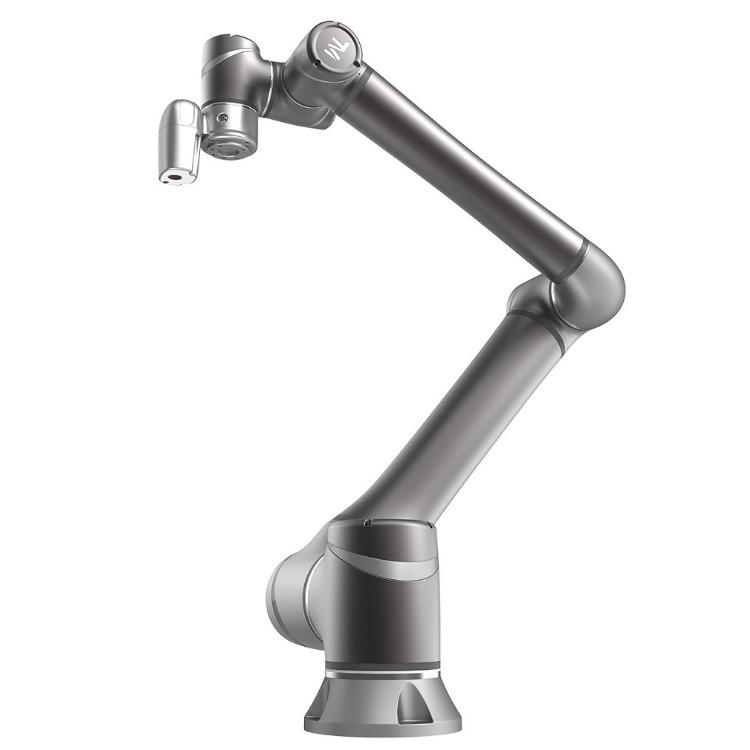
\includegraphics[width=0.5\textwidth]{./images/Chapter1/TechmanTM12}	
	\caption[ربات سری]{ربات سری \cite{SerialRobot}}
	\label{ربات سریال}
\end{figure}
\noindent
\unskip

\subsection{ربات‌های موازی}

به مرور زمان احساس نیاز به ســاختارهايي كه محدوديت‌هاي ربات‌های سـری را نداشـته باشند به وجود آمد. همانگونه كه ما انسان‌ها براي حركتهاي دقيق و يا برداشتن اجسام سنگين از هر دو دست خود استفاده مي‌كنيم، مي‌توان چنين تصـور كرد كه اسـتفاده از زنجيره‌هاي سـينماتيكي بسته كه چند بازو باهم و به صـورت موازي در حركت دخيل باشـند مي‌توانند پاسخي درخور براي اين مشكل باشد. 

همانطور که در شکل
\ref{ربات موازی}
مشاهده می‌شود ربات‌های موازي از زنجيره‌های بسـته سـينماتيكي سـاخته مي‌شوند كه شامل يك تكيه‌گاه
\noindent\unskip\LTRfootnote{Base}
و يك صفحه متحرك
\noindent\unskip\LTRfootnote{Moving Platform}
كه به وسيله تعدادي عملگر يا رابط به يكديگر متصل شده اند، مي باشد. مهمترين ضعف رباتهاي موازي محدوديت در فضاي كاری آنهاست. 
\begin{figure}[H]
	\centering
	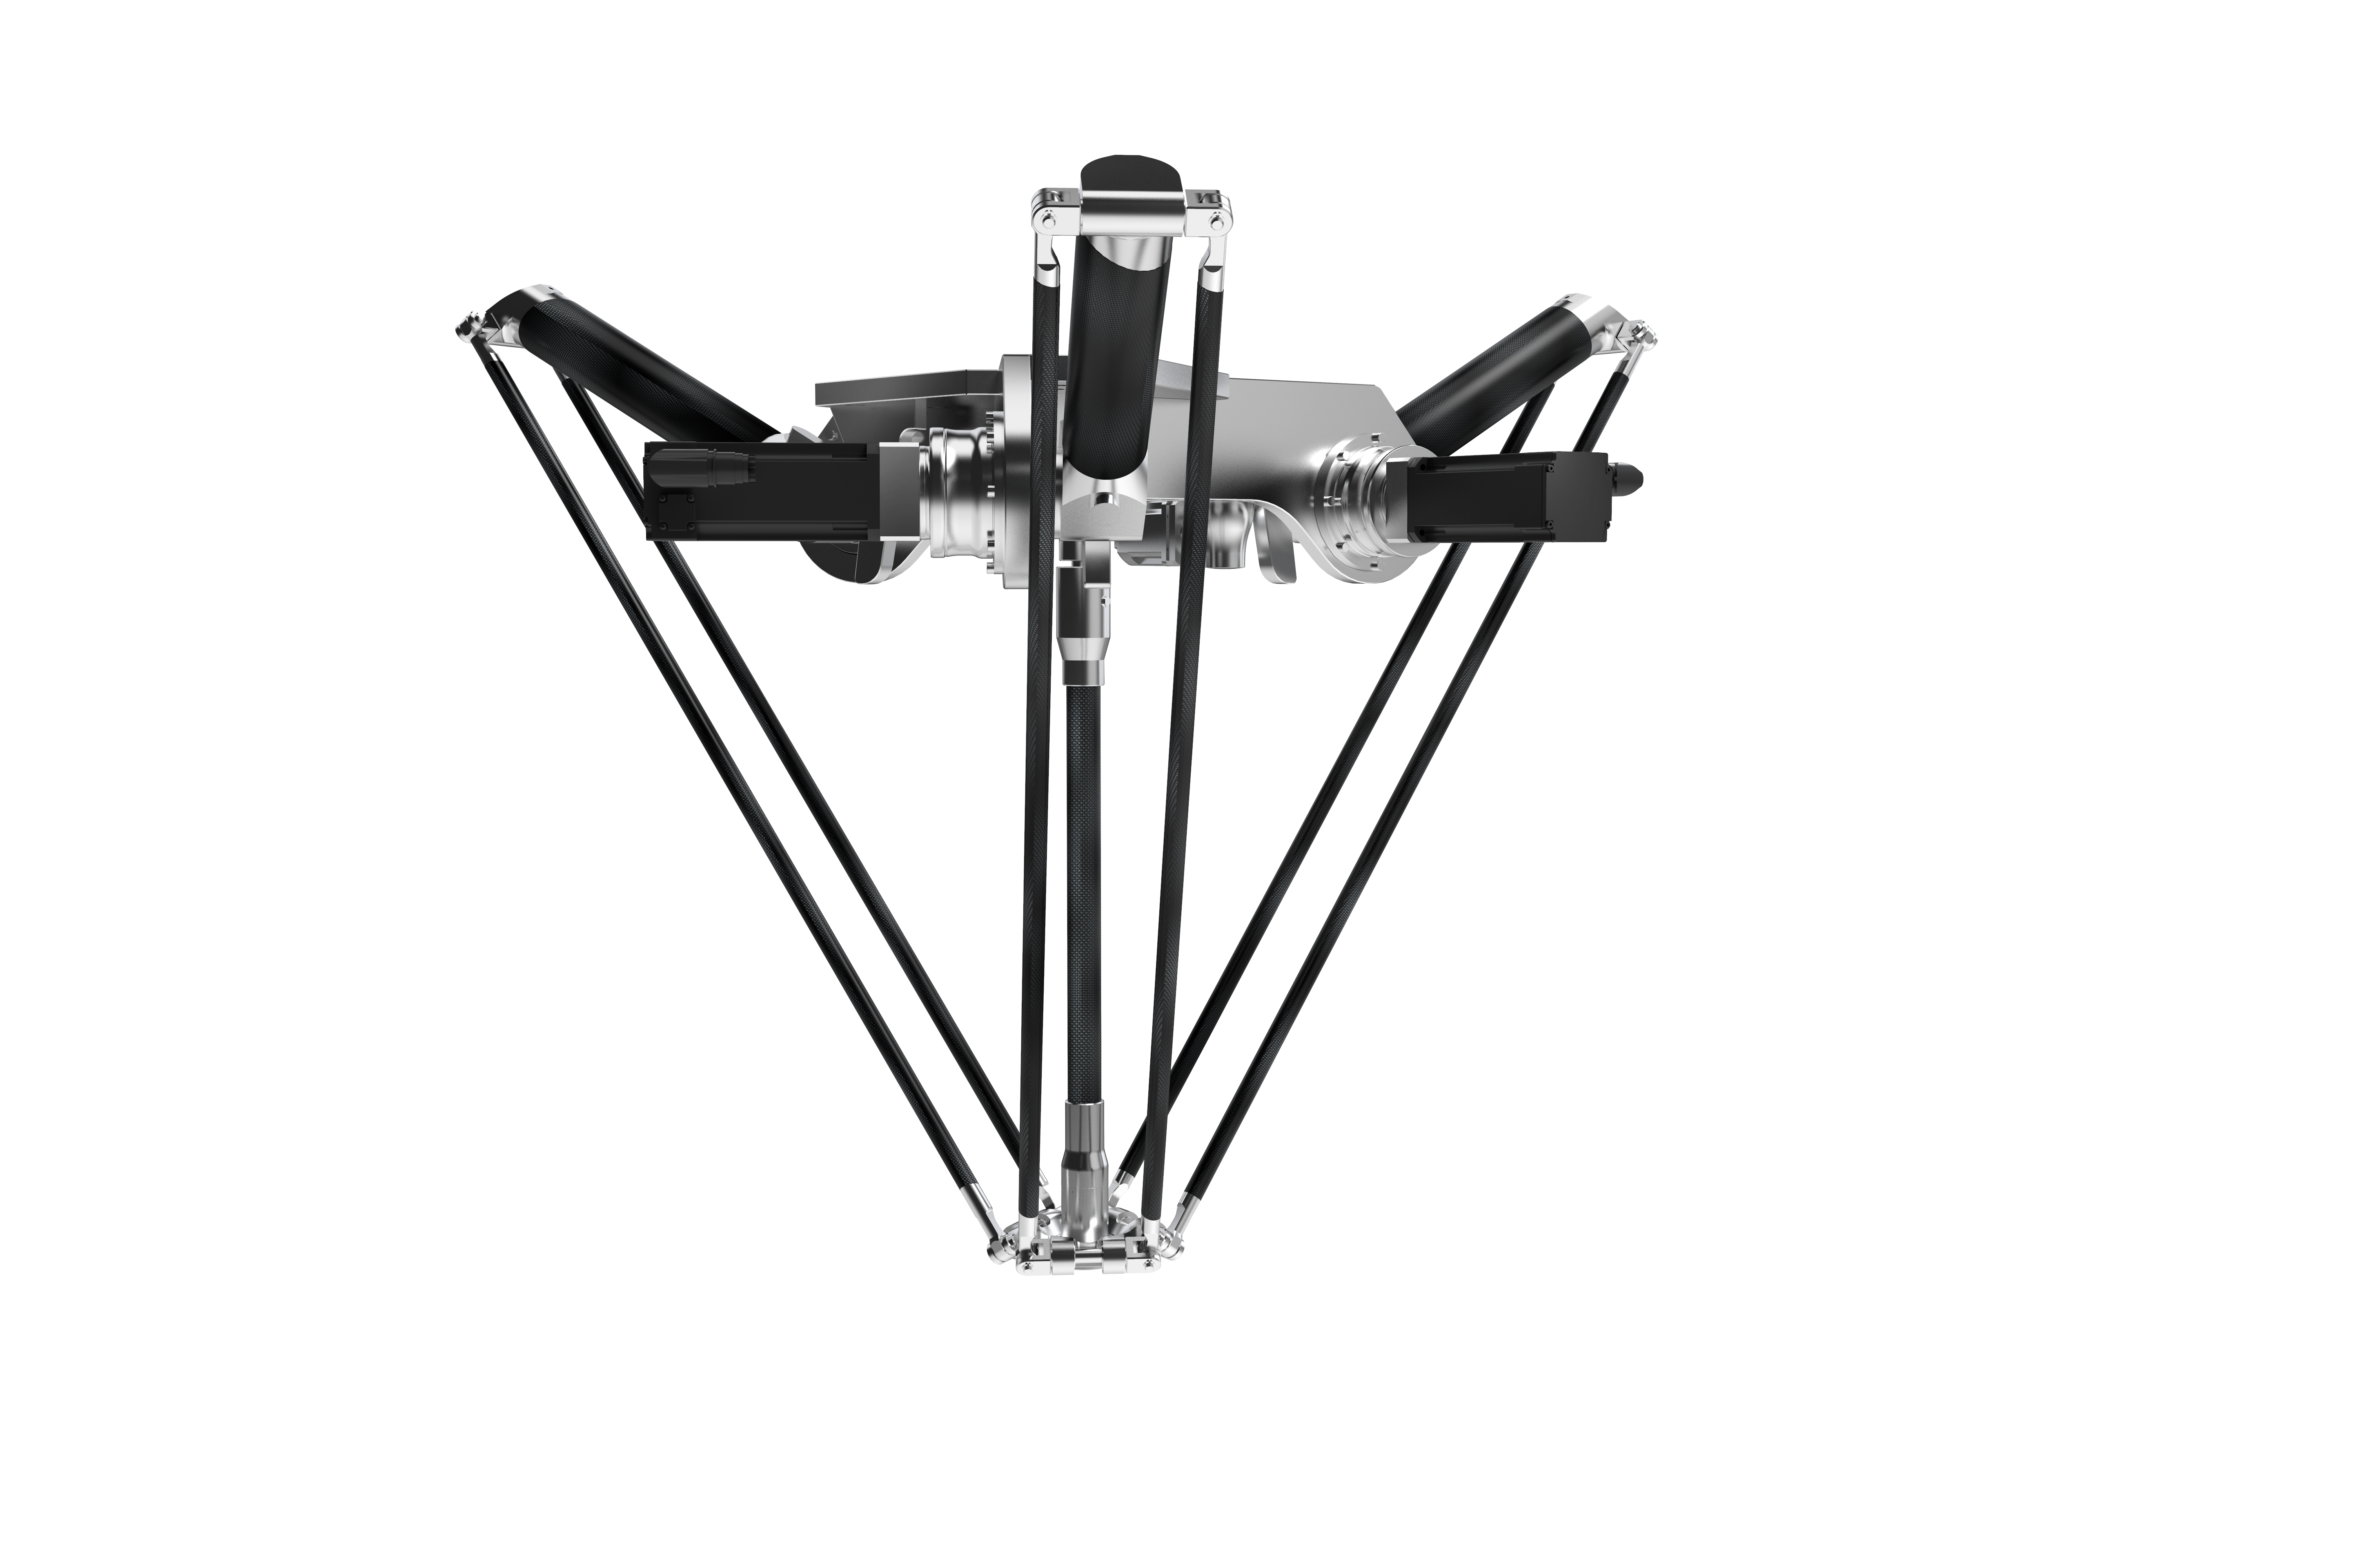
\includegraphics[width=0.5\textwidth]{./images/Chapter1/Delta2}	
	\caption[ربات موازی]{ربات موازی \cite{ParallelRobot}}
	\label{ربات موازی}
\end{figure}
\noindent
\unskip


\subsection{ربات‌های متحرک}
در دهه‌های اخیر، ربات‌های متحرک
\noindent\unskip\LTRfootnote{Mobile Robots}
به عنوان به عنوان ابزاری چندمنظوره و قدرتمند در دنیای مدرن از ماشین‌های خودکار تلقی می‌شوند. ربات‌های متحرک، از جمله دستاوردهای بزرگ در زمینه‌های مختلف از تحقیقات تا کاربردهای عملی، توانسته‌اند نقش مهمی را ایفا کنند. از تعقیب کاربردهای صنعتی تا خدمات انسانی و حتی مسائل محیط‌زیستی، علیرغم تنوع گسترده‌ی شکل‌ها و ساختارها، ربات‌های متحرک، توانایی انجام وظایف متنوع در محیط‌های مختلفی مانند صنایع کشاورزی، خدماتی و... را دارا هستند.
\begin{figure}[H]
	\centering
	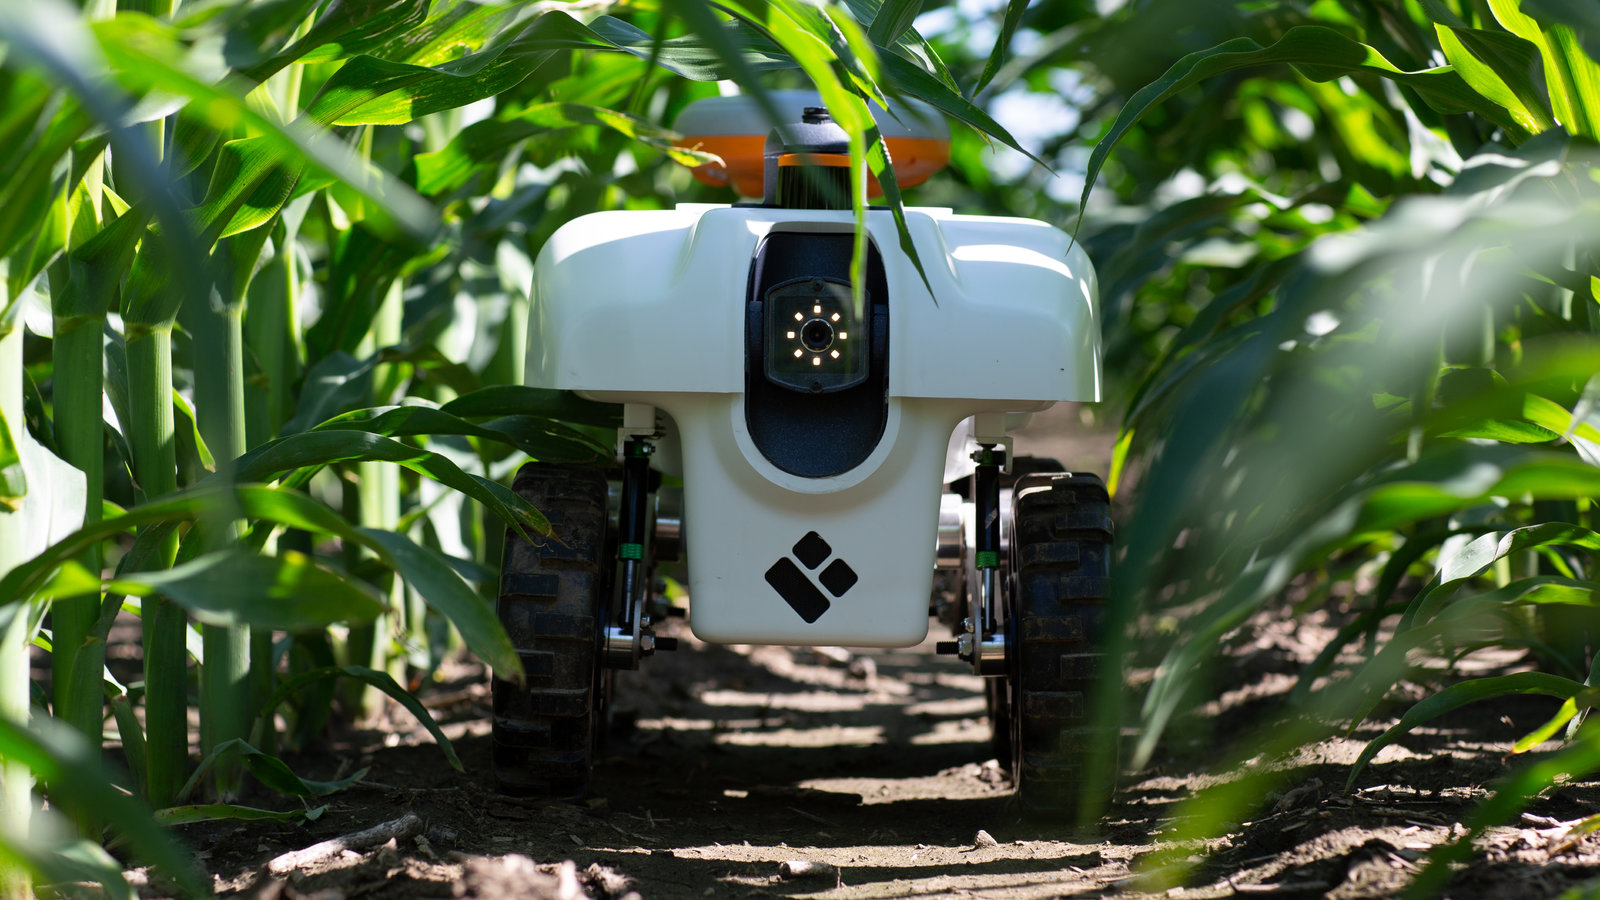
\includegraphics[width=0.5\textwidth]{./images/Chapter1/AgRobot}	
	\caption[ربات کشاورزی]{ربات کشاورزی \cite{AgRobot}}
	\label{ربات کشاورزی}
\end{figure}
\noindent
\unskip

ربات‌های متحرک در انواع مختلف طراحی می‌شوند که هر یک برای انجام وظایف خاصی از مکانیزم‌های متمایز استفاده می‌کنند. ربات‌های چرخدار
\noindent\unskip\LTRfootnote{Wheeled Robots}
، به عنوان مثال، از چرخ‌های محرک دارای موتورها برای حرکت و جابجایی استفاده می‌کنند. اینگونه ربات‌ها از استیکرهای تفاضلی بهره می‌برند که چرخ‌های موتورها در سمت‌های مختلف با سرعت‌های متفاوت می‌چرخند تا امکان تغییر جهت را فراهم کنند. 
ربات‌های پادار
\noindent\unskip\LTRfootnote{Legged Robots}
تلاش می‌کنند تا حرکت حیوانات را تقلید کنند و از پاها برای حرکت استفاده می‌کنند. کنترل ربات‌های پاهادار به دلیل درجات آزادی متعدد در مفاصل پیچیده‌است. ربات‌های هوایی مانند پهپادها، با استفاده از پره‌ها برای تولید لیفت و تراکم برای پرواز بهره می‌برند. این ربات‌ها نیاز به الگوریتم‌های کنترل پیچیده دارند تا پایداری و مسیر طی‌شده را مدیریت کنند.
\cite{Craig}

\section{ربات عنکبوتی چهارپا}
\subsection{ربات‌های عنکبوتی}
راه رفتن با چهار پا برای اکثر حیوانات رایج است و دلیل خوبی برای تکرار آن در ربات‌ها وجود دارد. ربات‌های عنکبوتی
\noindent\unskip\LTRfootnote{Spider Robots}
، از جمله انواع پیشرفته ربات‌ها، طراحی‌شده‌اند تا با تقلید از ساختار حرکت و عملکرد عنکبوت‌ها، قابلیت‌های منحصربه‌فردی در زمینه حرکت و کنترل را ارائه دهند. این ربات‌ها با دارا بودن چندین پا و قابلیت تحرک انعطاف‌پذیر، می‌توانند در محیط‌های مختلف و متغیر عملکرد خوبی داشته باشند. در ميان ربات هاي پادار، ربات هاي چهارپا به علت پايداري مناسب تر نسبت به ربات هاي دو‌پا و نيز تعداد پاهاي كمتر نسبت به ربات هاي شش پا، پيچيدگي كمتری را در طراحي و عمل دارند. ربات‌های چهارپا دارای پایداری استاتیکی هستند و الگوی راه رفتن یک ربات چهارپا را می‌توان به روش‌های مختلف طراحی کرد.

\begin{figure}[H]
	\centering
	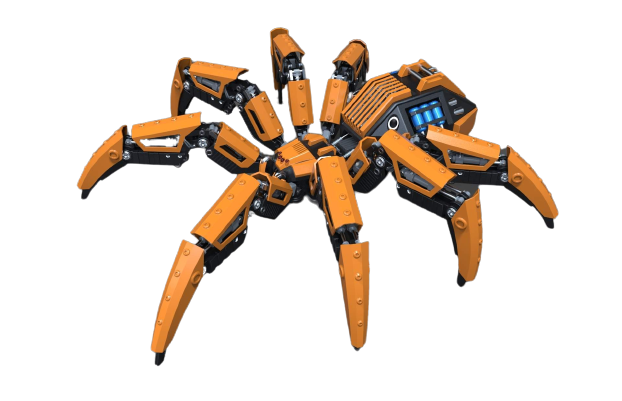
\includegraphics[width=0.5\textwidth]{./images/Chapter1/Spider2}	
	\caption[ربات عنکبوتی]{ربات عنکبوتی \cite{SpiderRobot}}
	\label{ربات عنکبوتی}
\end{figure}
\noindent
\unskip
در این پروژه، به بررسی ربات‌ عنکبوتی چهارپا می‌پردازیم که با تشکیل یک ساختار چهارپا و مکانیزم‌های تحرک پیچیده، قادر به مسیریابی و انجام وظایف متنوع در محیط‌ آزمایشگاهی می‌باشد.

\subsubsection{پایداری استاتیکی}

یک ربات با پایداری استاتیک تعادل خوبی دارد و در هنگام ایستادن به زمین نمی‌خورد. این بدین معنی است که مرکز ثقل ربات درون پایه تماس با زمین قرار دارد. فرض کنید یک ربات سه پا داریم که پاها به صورت مثلت تنظیم شده‌اند. این ربات تا زمانی‌که مرکز ثقل داخل مثلت قرار دارد، به هیچ نوع جابجایی برای ثابت ایستادن نیاز ندارد. این مثلث را «چند‌ضلعی حمایتی» می‌نامند که ناحیه‌ای افقی بالای مکان مرکز ثقل است تا پایداری استاتیک به دست آید. اگر جملات قبلی نامفهوم هستند، فقط کافی است متوجه شوید که چندضلعی حمایتی همان سطحی است که ربات روی آن ایستاده و درون نقاط حمایتی قرار دارد.

\begin{figure}[H]
	\centering
	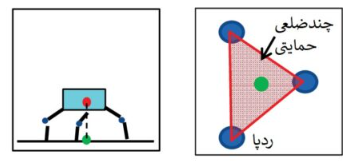
\includegraphics[width=0.5\textwidth]{./images/Chapter1/StaticStability}	
	\caption[پایداری استاتیکی]{چندضلعی حمایتی \cite{StaticStability}}
	\label{پایداری استاتیکی}
\end{figure}
\noindent
\unskip



\subsection{ربات‌های عنکبوتی چهارپا}
ربات‌های عنکبوتی چهارپا
\noindent\unskip\LTRfootnote{Quadruped Spider Robots}
، با شباهت به حرکت عنکبوت‌های طبیعی، به کمک چهار پا محرک تحرک کرده و قادر به تغییر شکل در محیط‌های مختلف هستند. این انعطاف‌پذیری در حرکت، به ربات‌ها امکان حرکت در مسیرهای مختلف، شکل گیری برای عبور از موانع و تطابق با محیط را می‌دهد. علاوه بر این، استفاده از حسگرهای چندگانه مانند دوربین‌ها، ژیروسکوپ‌ها و... به ربات‌ها امکان مشاهده و تجزیه و تحلیل محیط را می‌دهد. این قابلیت‌ها به عنوان اصول مهم در ناوبری، پیمایش محیط و انجام وظایف متنوع در برنامه‌ریزی و کنترل ربات‌های عنکبوتی چهارپا مورد استفاده قرار می‌گیرد.
برای درک بهتر یک نمونه از ربات‌های عنکبوتی چهارپا که در واقع همان ربات پایان‌نامه پیش روست و طراحی اولیه آن در محیط سالیدورک انجام شده‌است، در شکل 
\ref{نسخه‌اولیه }
قابل مشاهده می‌باشد.

\begin{figure}[H]
	\centering
	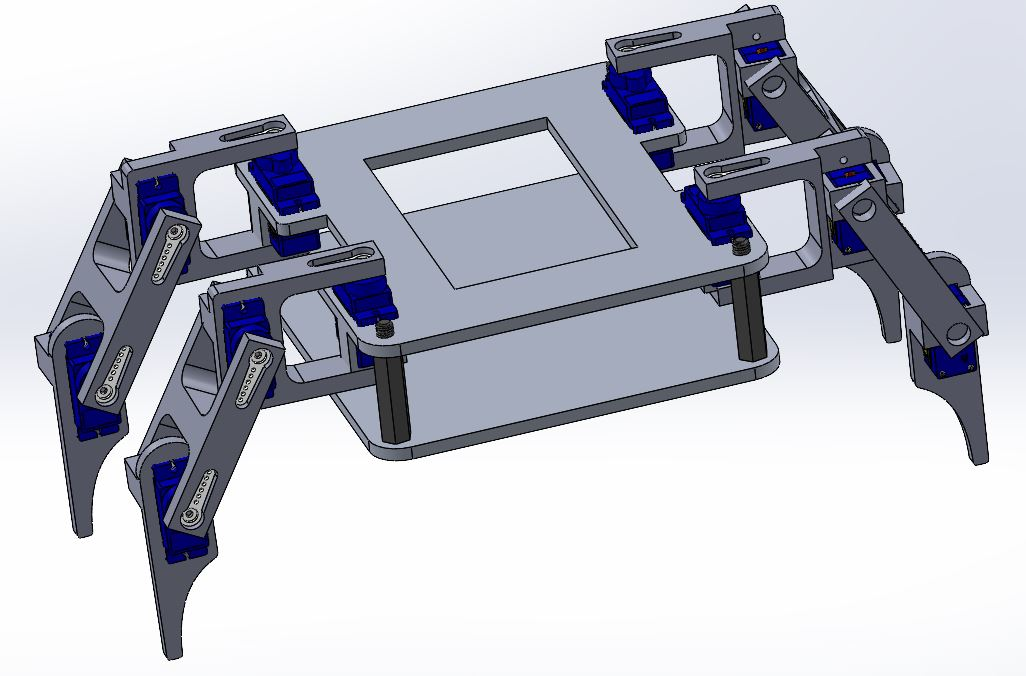
\includegraphics[width=0.6\textwidth]{./images/Chapter1/Robot_Final}	
	\caption[نسخه‌اولیه طراحی شده]{نسخه‌اولیه طراحی شده}
	\label{نسخه‌اولیه }
\end{figure}
\noindent
\unskip

\section{تاثیر هوش مصنوعی بر رباتیک}

در دهه‌های اخیر، پیشرفت‌های چشمگیری در زمینه هوش مصنوعی و رباتیک ایجاد شده است که به‌طور گسترده تأثیرات قابل‌توجهی را در صنعت و علم رباتیک ایجاد کرده است. هوش مصنوعی به عنوان یکی از شاخه‌های علوم کامپیوتر که در تلاش برای تجسم و شبیه‌سازی هوش انسانی بوده و همچنین توانایی یادگیری و تصمیم‌گیری در ماشین‌ها را دارد.

ترکیب هوش مصنوعی با رباتیک، باعث پدیدآمدن ربات‌های هوشمند و تعاملی شده است که توانایی‌هایی انسان‌نمایانه از جمله تشخیص محیط، پردازش اطلاعات، تصمیم‌گیری و انجام وظایف پیچیده را اجرا می‌کنند. این ترکیب موجب ایجاد امکانات جدید در زمینه‌های مختلف مانند صنعت، پزشکی، کشاورزی هوشمند، خودروهای خودران و بسیاری دیگر شده‌است.

در این پایان‌نامه به بررسی اثرات هوش مصنوعی بر رباتیک در یک نمونه خاص از ربات‌ها (ربات چهارپا) و همچنین کاربردها و چالش‌های متنوعی که این ترکیب مهارت‌ها ایجاد می‌کنند، پرداخته خواهد شد. این نمونه خاص‌ از ربات‌ها مثال خوبی از تعامل موثر هوش مصنوعی و روباتیک در مختلف زمینه‌ها می‌پردازد.

\section{مروری بر الگوریتم‌های مسیریابی}\label{مروری بر الگوریتم‌های مسیریابی}

امروزه با ساخت ربات‌های مختلف، برنامه مساله‌ریزی مسیر ربات، بسیار
مورد توجه قرار گرفته است. به طور خلاصه، مساله برنامه‌ریزی مسیر،
یافتن مسیری است که ربات را از نقطه شروع به نقطه هدف هدایت
می‌کند.
\cite{}
در بسیاری از کاربردها برای اینکه ربات بتواند وظیفه خود را
بدرستی انجام دهد، نیاز به حرکت در محیط دارد. الزام حرکت در محیط موجب پرسیدن این سوال می‌شود که، ربات برای انجام وظیفه خود چه مسیری را طی کند که علاوه بر ایمن بودن آن، با کمترین هزینه به هدف خود برسد. با توجه به محدودیت انرژی، تسریع در انجام کارها و عدم
برخورد ربات با موانع موجود در محیط، اهمیت این سوال بهتر درک می‌شود. پاسخگویی به این پرسش، که پرسش اساسی در زمینه تحقیقاتی مهمی تحت عنوان برنامه‌ریزی مسیر است، از دیدگاه‌های مختلف صورت گرفته است.

رویکردهای حل برنامه مسئله ریزی مسیر را می‌توان به چند دسته کلی تقسیم کرد:
\begin{enumerate}
	\item
	بلادرنگ: اگر ربات از وقایع محیطی، مکان و حرکت موانع، از قبل اطلاع نداشته باشد، آنگاه به یافتن مسیری ایمن به سوی هدف مبادرت کند، در این حالت برنامه‌ریزی بلادرنگ نامیده می‌شود.
	\cite{}
	\item
	کامل و کامل احتمالاتی: ارائه یک مسیر، در صورت وجود، کامل بودن
	الگوریتم نامیده می‌شود. کامل بودن احتمالاتی نیز به این معنی است که اگر الگوریتم تا زمان طولانی اجرا شود، در صورت وجود یک مسیر، آن را خواهد یافت.
	\cite{}
	
\end{enumerate}

از جمله روش‌های مطرح برای حل برنامه مساله‌ریزی مسیر،
الگوریتم‌های مبتنی برنمونه‌گیری هستند. در این روش‌ها با نمونه‌برداری از فضای پیکربندی، به ساخت درختی از نقطه شروع، مبادرت می شود. با رسیدن یکی از شاخه‌های درخت به نقطه هدف الگوریتم خاتمه می یابد.
 این روش در ابتدا توسط
\lr{Lavalle}
در سال 1991 تحت عنوان درخت جستجوی سریع تصادفی
\lr{RRT}
مطرح گردید.
% \section{برنامه ریزی مسیر}
% \subsection{تاریخچه برنامه ریزی مسیر}

% در این بخش به تاریخچه برنامه‌ریزی مسیر می‌پردازم.
% \subsection{مفهوم برنامه ریزی مسیر}

% در این بخش به مفهوم برنامه‌ریزی مسیر می‌پردازم.


\section{اهداف و نوآوری}

با نگاهی به پژوهش هاي انجام شده در زمينه ربات هاي عنکبوتی چهارپا مشاهده می‌شود كه در اكثر پژوهش هاي صورت گرفته به ديدگاه تئوري بيشتر اهمیت داده شده‌است. از این رو در پژوهش پيش رو تلاش شده است تا جنبه‌های عملی ربات‌‌های پادار مورد توجه قرار گرفته و همچنین تمرکز بر روی بهبود عملکرد و افزایش قابلیت‌های آنها گردد. در نتیجه این هدف، با انتخاب مکانیزمی سهل‌تر برای حرکت در محیط، به انجام وظایف محوله توسط ربات پرداخته شده‌است.
از مهمترین نوآوری این پژوهش، می‌توان به موارد زیر اشاره کرد:
\begin{itemize}
	\item
	افزودن دوربین به ربات به منظور تشخیص موانع مختلف موجود در محیط
	\item
	مانیتورینگ بلادرنگ
	\noindent\unskip\LTRfootnote{Real Time}
	تصویر محیط
	\item
	مدیریت برخط
	\noindent\unskip\LTRfootnote{Online}
	اطلاعات ارسالی از محیط به ربات و بالعکس
\end{itemize}

% اطلاعات ارسالی بر روی سرور می‌باشد.

\section{ساختار پایان نامه}

پس از اتمام پایان نامه روند هر بخش را مختصرا توضیح خواهم داد.
\newpage
\section{جمع بندی}

با توجه به طراحی اولیه برای ربات و بررسی قابلیت‌های قابل ارتقا، تمرکز اصلی بر روی بهبود مداوم و حداکثری ربات (از لحاظ نکات طراحی و ساخت و همچنین بخش نرم‌افزاری آن)در طی مراحل مختلف قرار گرفت. در نهایت با ساخت نمونه اولیه و اسمبل
\noindent\unskip\LTRfootnote{Assemble}
شدن آن به شروع جدی‌تر بخش نرم‌افزار و برطرف کردن چالش‌های عملی آن پرداخته شد.
نمونه اسمبل شده اولیه ربات در شکل
\ref{نسخه‌اسمبل شده}
قابل مشاهده می‌باشد.

\begin{figure}[H]
	\centering
	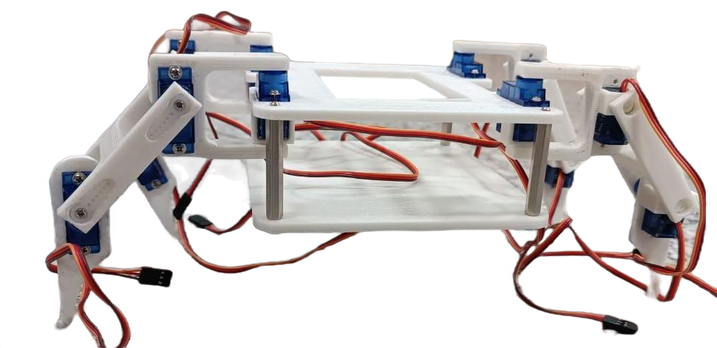
\includegraphics[width=0.5\textwidth]{./images/Chapter1/Assembled_Robot_without_background}	
	\caption[نسخه‌اسمبل شده]{نسخه‌اسمبل شده}
	\label{نسخه‌اسمبل شده}
\end{figure}
\noindent
\unskip

\chapter{مسیریابی و الگوریتم های پیاده سازی شده}

\section{مقدمه}

در این فصل پایان‌نامه به پردازش تصویر و ارتباط بین ربات و سرور می‌باشد. این فصل به معرفی و بررسی اصول و مبانی پردازش تصویر و نیز نحوه‌ی ارتباط و تبادل اطلاعات بین ربات چهارپا و سرور می‌پردازد. در دنیای امروز که هوش مصنوعی و فناوری‌های رباتیک و در حال پیشرفت های صنعتی می‌باشند، تلفیق پردازش تصویر به عنوان یک افزونه از ربات و ارتباط میان ربات و سرور، برای انجام وظایف پیچیده و کاربردهای متنوع بسیار حائز اهمیت می‌باشد.

این فصل به بررسی مفاهیم پایه پردازش تصویر، تکنیک‌های استخراج و تحلیل اطلاعات از تصاویر، و همچنین نحوه‌ی ارتباط بین ربات و سرور اختصاص دارد. از جمله مسائل مورد بررسی در این فصل، می‌توان به پیش‌پردازش تصاویر، تشخیص الگوها، تصویرسازی داده‌ها و ارسال اطلاعات بین ربات و سرور اشاره کرد.

به عنوان پایه‌ای برای فصل‌های بعدی، این فصل به ما امکان می‌دهد تا اصول پایه پردازش تصویر را برای کنترل و هدایت ربات‌ها بهره‌برداری کنیم. همچنین، اهمیت برقراری ارتباط مؤثر بین ربات و سرور را برای جمع‌آوری داده‌ها و انتقال دستورات کنترلی تاکید می‌کند.

در این فصل، ابتدا به مقدمه‌ای کوتاه درباره موضوع، اهمیت و اهداف این فصل می‌پردازیم. سپس به توضیح دقیق‌تر مفاهیم پایه پردازش تصویر و ارتباطات ربات و سرور می‌پردازیم. در پایان نیز ساختار و مرور مطالب فصل‌های آینده را معرفی خواهیم کرد.

با توجه به اهمیت این فصل در ساختار کلی پایان‌نامه و کاربردهای آینده، مطالب ارائه شده در این فصل بهترین پایه‌ها و مفاهیم را برای فهم بهتر و تحلیل دقیق‌تر موضوعات بحرانی در پژوهش ارائه خواهد داد.
\section{مقدمه‌ای بر پردازش تصویر}
\section{پردازش تصویر}
\subsection{مقدمه}

از مهمترین موضوعات هوش مصنوعی که در سال های اخیر حوزه‌های مختلف به ویژه مهندسی را تحت تاثیرات بسزایی قرار داده‌است، می‌توان به پردازش تصویر و بینایی ماشین اشاره کرد. کاربردهای کنترلی همچون ماشین‌های خودران، دوربین‌های کنترل جرایم رانندگی، سیستم‌های تشخیص چهره و... از پردازش تصویر بهره می‌برند.
\subsection{تصویر چیست؟}

تصویر، نوعی نمایش بصری از داده‌هاست که معمولاً توسط دوربین‌ها یا سنسورهای تصویربرداری ثبت می‌شود.تصویر به صورت مجموعه‌ای از نقاط کوچک به نام پیکسل‌ها تشکیل می‌شود که هر کدام حاوی اطلاعاتی چون رنگ و روشنایی می‌باشند. از طریق ترکیب مختلف پیکسل‌ها، تصویرهایی با پیچیدگی، اشکال و جزئیات مختلف ایجاد می‌شوند.

تصاویر می‌توانند در انواع مختلف از جمله تصاویر رنگی، تصاویر سیاه و سفید و... باشند. از تصاویر به عنوان یک ابزار قوی برای انتقال اطلاعات و نمایش داده‌ها در زمینه‌های مختلف از جمله در پزشکی، هنر، رباتیک و...استفاده می‌شود.
\subsection{پردازش تصویر چیست؟}

پردازش تصویر یک زیرشاخه از پردازش سیگنال است که به تحلیل، تغییر، و بهبود تصاویر دیجیتالی می‌پردازد. در این فرآیند، تصاویر از دوربین‌ها یا سنسورهای تصویربرداری گرفته می‌شوند و سپس توسط الگوریتم‌ها و روش‌های پردازشی مختلف تجزیه و تحلیل می‌شوند.

هدف اصلی پردازش تصویر بهینه‌سازی و تحسین کیفیت تصاویر است. این می‌تواند شامل کاهش نویز، تعدیل رنگ و کنتراست، تشخیص الگوها، تشخیص ویژگی‌ها و استخراج اطلاعات از تصاویر باشد. در زمینه‌های مختلف از پردازش تصویر استفاده می‌شود که از جمله آنها می‌توان به پزشکی (تشخیص بیماری‌ها از تصاویر پرتونگاری)، رباتیک (شناسایی محیط توسط ربات‌ها)، و امنیت (تشخیص چهره‌ها و اجسام در تصاویر نظارتی) اشاره کرد.

پردازش تصویر شامل مراحل مختلفی مانند پیش‌پردازش، تبدیلات، تشخیص الگوها، و استخراج ویژگی‌ها است. الگوریتم‌های پردازش تصویر معمولاً بر اساس مفاهیم ریاضی، آمار و هوش مصنوعی طراحی می‌شوند. از این رو می‌توان گفت پردازش تصویر در حوزه‌های مختلف از مهندسی، علوم رایانه، و علوم پایه کاربردهای متعددی داشته و از اهمیت بالایی در تحلیل و انتقال اطلاعات تصویری برخوردار است.

\section{الگوریتم جستجوی سریع درخت تصادفی}
\subsection{مقدمه}
همانطور که در بخش
\ref{مروری بر الگوریتم‌های مسیریابی}
اشاره شد، الگوریتم‌های متنوعی در رباتیک کاربرد دارد.

در حوزه‌ی رباتیک، پیشرفت‌های قابل توجهی در الگوریتم‌های برنامه‌ریزی مسیر رخ داده است که به ربات‌های خودکار امکان می‌دهد تا به طور کارآمد در محیط‌های پیچیده حرکت کنند. از میان این الگوریتم‌ها، الگوریتم 
\textbf{جستجوی سریع درخت تصادفی}
\noindent\unskip\LTRfootnote{Rapidly Exploring Random Tree}
یا به اختصار
\lr{RRT}
به عنوان یک رویکرد نوآورانه شناخته می‌شود که به حل چالش یافتن مسیرهای قابل اجرا در فضاهای تنظیم با بعد بالا می‌پردازد. این الگوریتم به عنوان یک روش مبتنی بر هیوریستیک
\noindent\unskip\LTRfootnote{Heuristic}
، با استفاده از تصادف و کاوش به سرعت یک ساختار مانند درخت را ایجاد می‌کند که این امر آن را برای کاربردهای بهینه‌سازی زمان و محیط‌های پویا مناسب می‌کند. اصول اساسی این الگوریتم در قابلیت اکتشاف مؤثر فضاهای تنظیمی و تنوع آن، آن را به یک اصول اصلی در تحقیقات و کاربردهای رباتیک مدرن تبدیل کرده است.

الگوریتم
\lr{RRT}
که در حوزه‌ی برنامه‌ریزی حرکت معرفی شده است، یک راه حل نوین برای چالش پیچیده یافتن مسیر برای عوامل خودکار در فضاهای با بعد بالا ارائه می‌دهد. در اصل، این روش به دنبال برقراری تعادل بین کاوش و بهره‌برداری می‌گردد. این الگوریتم با یک تنظیم اولیه آغاز می‌شود و به صورت تکراری با نمونه‌برداری تصادفی از نقاط در فضای تنظیمی، آن‌ها را به نزدیک‌ترین نقطه در درخت موجود متصل می‌کند. این رویکرد تضمین می‌کند که الگوریتم مناطقی از فضا را که هنوز کاوش نشده‌اند، کاوش کند، در عین حال به طور تدریجی از مناطقی که قبلاً کاوش شده‌اند بهره‌برداری می‌کند.

یکی از ویژگی‌های برجسته‌ی
\lr{RRT}
توانایی تطبیق به محیط‌ها و محدودیت‌های مختلف است. با تشکیل تک تک نقاط درخت به طور تدریجی، رشد الگوریتم به سمت مناطقی با کاوش کمتر سوق می‌شود، که این ویژگی آن را به ویژه برای موقعیت‌هایی که فضای تنظیم مشخص نشده یا با موانع پراکنده است، مناسب می‌کند. علاوه بر این،
\lr{RRT}
همگام‌سازی سریع را اجرا می‌کند که به آن اجازه می‌دهد که مسیرهای قابل اجرا را به سرعت ایجاد کند، حتی در محیط‌های پیچیده و پویایی.

قابلیت‌های این الگوریتم در کاربردهای زمان‌واقع واقعی نیز یک جنبه جذاب دیگر است. به دلیل ساختار تکراری و تطبیق‌پذیری، این الگوریتم برای مواردی که تصمیم‌گیری باید سریع و واکنش‌پذیر باشد، مناسب است. علاوه بر این، محققان اقدام به توسعه
\lr{RRT}
برای مواجهه با چالش‌های خاص، مانند موانع پویا و سیستم‌های چندعاملی و... کرده‌اند که بیشتر نشان می‌دهد چقدر این الگوریتم چندمنظوره و عملی است.

به عبارتی، الگوریتم
\lr{RRT}
یک الگوریتم نوآورانه برای برنامه‌ریزی مسیرهای خودکار است. با ترکیب کاوش و بهره‌برداری ،
\lr{RRT}
به طور موثر در فضاهای تنظیمی با بعد بالا حرکت کرده و به شکل مناسبی به شرایط محیطی مختلف تطبیق می‌یابد. چندمنظورگی، قابلیت‌های زمان‌واقع و تطبیق‌پذیری با چالش‌های خاص،
\lr{RRT}
را به یک ابزار ارزنده در تحقیقات و کاربردهای رباتیک مدرن تبدیل کرده است و پیشرفت‌هایی در خودکاری، کارایی و ایمنی ایجاد می‌کند.


\subsection{شبیه‌سازی دوبعدی با پایتون}
\subsubsection{نتایج شبیه‌سازی}
در ابتدا نتایج حاصل از شبیه‌سازی توسط پایتون قرار داده‌ شده‌است. همانطور که در شکل
\ref{نتیجه شبیه‌سازی RRT}
قابل مشاهده است، یک محیط با ابعاد مشخص و تعداد موانع مشخص طراحی و سپس با تعیین نقطه شروع و پایان برای ربات، با استفاده از الگوریتم پیشنهادی ربات توانسته است مسیر خود را بدون برخورد با موانع بیابد.
\begin{figure}[H]
	\centering
	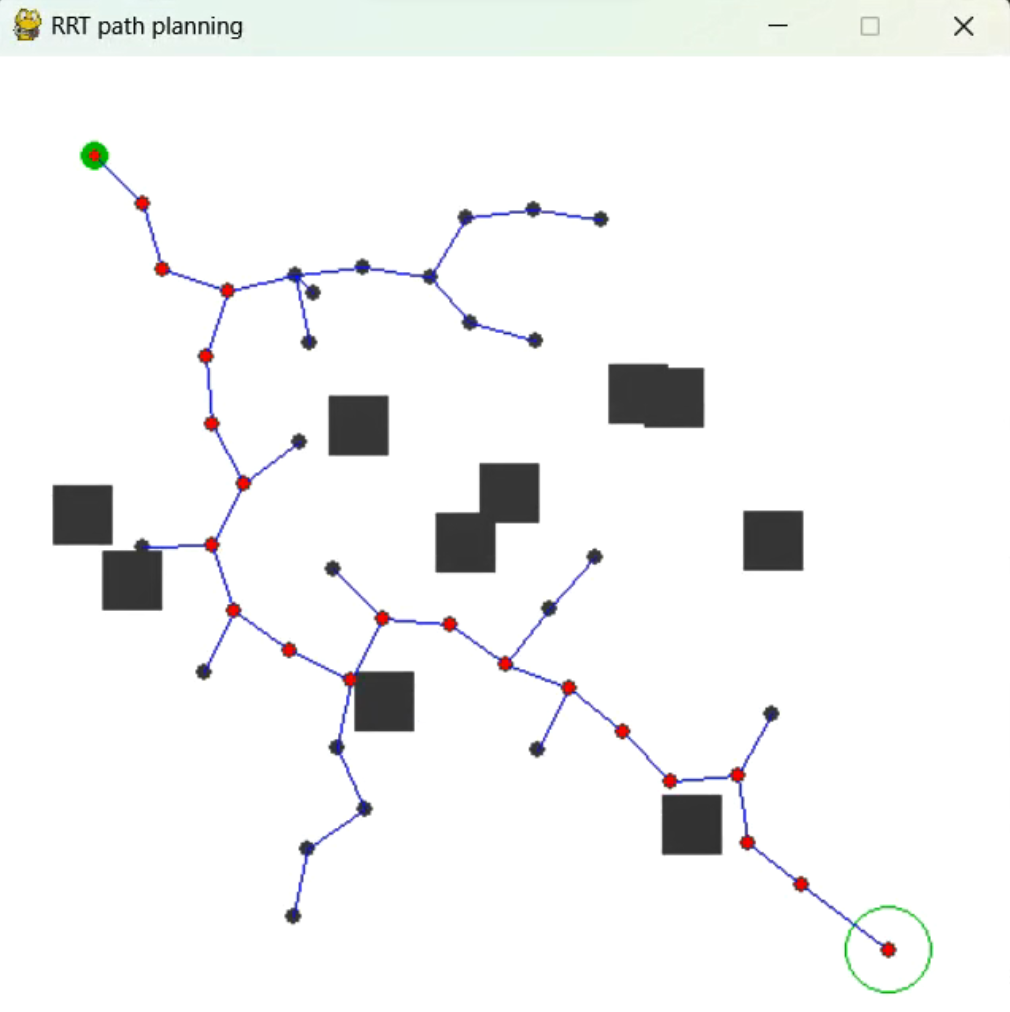
\includegraphics[width=0.7\textwidth]{./images/Chapter2/ConvexResult}	
	\caption[شبیه سازی الگوریتم \lr{RRT}]{شبیه سازی الگوریتم \lr{RRT}}
	\label{نتیجه شبیه‌سازی RRT}
\end{figure}
\noindent
\unskip

\subsubsection{شبیه‌کد و تشریح جزئیات برنامه}
در زیر شبه‌کد این بخش مختصرا قراره داده شده و پس از آن به تشریح کامل‌تر آن پرداخته خواهد شد.
\section*{}
\begin{latin}
	\lstinputlisting[style=python_style]{code/Pseudocodes/RRTPseudocode.py}
\end{latin}

همانطور که در شبه‌کد بالا مشخص است برنامه تا زمانی که آخرین گره گراف به ناحیه نزدیک نقطه هدف نرسد ادامه خواهد داشت. جزئیات و نحوه تولید مسیر در قطعه برنامه‌ای در پیوست موجود می‌باشد. نحوه عملکرد توابع اصلی برنامه برای تولید مسیر به شرح زیر است:
\begin{itemize}
	\item
	تولید یک گره تصادفی با فاصله مشخص از گره شروع
	\item
	بررسی معتبر بودن گره جدید (معتبر بودن به معنای آنکه آیا گره جدید بر روی موقعیت یکی از موانع نبوده باشد.)
	\item
	در صورت معتبر بودن گره جدید با فواصل از پیش تعیین شده توسط چند قدم یال‌هایی برای گراف ایجاد می‌شود.
	\item
	اگر در طی این چند قدم یکی از یال‌ها با یکی از موانع برخورد داشته باشد، قدم دیگری برای رسیدن به گره جدید انتخاب می‌شود. در غیر این صورت برنامه تا رسیدن به گره جدید ادامه داده و دوباره به مرحله اول(تولید گره تصادفی) برگشت داده خواهد شد.
\end{itemize}

\begin{figure}[H]
	\centering
	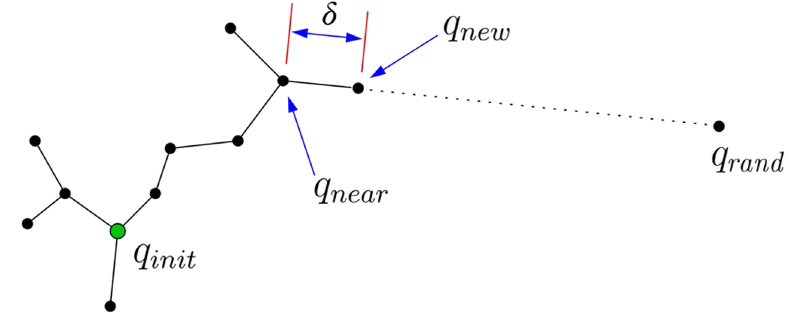
\includegraphics[width=0.8\textwidth]{./images/Chapter2/NewNodeSteps_without_background}	
	\caption[مراحل تولید گره جدید و تشکیل مسیر]{مراحل تولید گره جدید و تشکیل مسیر\cite{Algobotics}}
	\label{مراحل تولید گره جدید}
\end{figure}
\noindent
\unskip

برای درک بهتر مراحل بالا می‌توان شکل
\ref{مراحل تولید گره جدید}
را در نظر گرفت. همچنین قابل ذکر است که برای هر یک از مراحل بالا یک یا دو متد
\noindent\unskip\LTRfootnote{Method}
در ماژول نوشته شده در نظر گرفته شده است و این متد‌ها با یکدیگر در ارتباط بوده و یا به صورت تو در تو
 \noindent\unskip\LTRfootnote{Nested}
در یکدیگر استفاده شده‌اند. 

\subsubsection{ادغام الگوریتم با قابلیت‌های ربات به منظور پیاده‌سازی}
همانطور که مشخص است استفاده از الگوریتم پیشنهادی به تنهایی مفید واقع نخواهد شد و بایستی از قابلیت های موجود در ربات برای بهینه‌سازی این روش استفاده شود. از قابلیت های ربات که می‌تواند به کار آید، دوربین استفاده شده می‌باشد. با استفاده از دوربین موجود موانع و فاصله‌ی ربات تا موانع تشخیص داده شده و سپس با توجه به این اطلاعات ربات تصمیم می‌گیرد تا نقاط تصادفی خود را در کدام جهت تولید کند و یا در کدام جهت به تولید ادامه مسیر نپردازد. بدین منظور در بخش های آتی به تشریح موارد ذکر شده پرداخته خواهد شد.

\newpage
\section{\lr{Localization}}

\subsection{مقدمه}

مکان‌یابی یکی از جنبه‌های حیاتی در علم رباتیک است که به ربات‌ها امکان می‌دهد تا مکان و موقعیت دقیق خود را در محیط تعیین کنند. برای ربات‌ها، داشتن اطلاعات صحیح و دقیق در مورد مکان خود بسیار مهم است تا بتوانند به درستی عمل کرده و وظایف مختلفی را انجام دهند. در اینجا، ما به مکان‌یابی در رباتیک می‌پردازیم و نحوه استفاده از تگ‌های
\lr{Aruco}
را برای تعیین موقعیت دقیق ربات توضیح خواهیم داد.


\subsection{استفاده از تگ}
بدانید که مکان‌یابی در رباتیک به وسیله مختصات مکانی (مثلاً نقاط (x، y، z) یا مختصات خروجی (طول، عرض، ارتفاع) صورت می‌پذیرد. این اطلاعات توسط تگ‌های "Aruco" به ربات ارائه می‌شود. این تگ‌ها اطلاعاتی را شامل می‌شوند که شامل سه زاویه (roll، pitch، yaw) برای جهت‌یابی و فاصله‌ها در سه محور مختلف می‌شوند. برای دقت بیشتر در محاسبات، ما یک ماتریس را تعریف می‌کنیم که حاوی فاصله‌های مرکزی دوربین و فوکوس آن است و این ماتریس را به کد مکان‌یابی ارائه می‌دهیم. این اطلاعات به ربات امکان می‌دهند تا موقعیت و جهت خود را با دقت بیشتری تعیین کنند و وظایف خود را انجام دهند.
\subsubsection{مقدمه}

\section{جمع بندی}


\chapter{نرم ‌افزار و ارتباطات}
\label{chapter3}
\section{ارتباطات و سرور}

\subsection{اتصال بیسیم دوربین به سرور}

%در این بخش از پایان‌نامه، به توضیح نحوه اتصال ماژول ESP32 CAM به روتر از طریق کد آردوینو و همچنین توضیح نوشتن یک مدیر دستگاه برای سرور در فایل apphttpd.cpp می‌پردازیم.% 
\subsubsection{مفاهیم اصلی}
در این بخش به تبیین مفاهیمی از شبکه
\noindent\unskip\LTRfootnote{Network}
که مورد استفاده قرار گرفته اند و تشریح فرآیندهای انجام شده برای برقراری ارتباط بین ماژول
\lr{ESP32 CAM} 
و سرور پرداخته شده‌است. در شبکه‌های اینترنتی دو مفهوم پرکاربرد با کلیدواژه نقطه دسترسی
\noindent\unskip\LTRfootnote{Access Point}
و مُد
\noindent\unskip\LTRfootnote{Mode}
ایستگاهی
\noindent\unskip\LTRfootnote{Station}
(یا به اختصار
\lr{STA})
وجود دارد. 
طبق تعریف، نقطه دسترسی
\cite{AccessPoint}
یک دستگاه سخت افزاری شبکه‌است که به سایر دستگاه ها اجازه می‌دهد به یک شبکه سیمی متصل شوند و به عنوان یک دستگاه مستقل، ممکن است یک اتصال سیمی به یک روتر
\noindent\unskip\LTRfootnote{Router}
داشته باشد. اگرچه در یک روتر بی سیم، می تواند جزء جدایی ناپذیر خود روتر نیز باشد.


احتمالا تجربه متصل کردن تلفن همراه و یا سایر وسایل الکترونیکی خود به مودم خانگی را داشته اید. در این حالت تلفن همراه در مُد ایستگاهی جهت دریافت آی پی
\noindent\unskip\LTRfootnote{Internet Protocol address}
از مودم و همچنین مودم نیز در حالت نقطه دسترسی قرار گرفته‌است. به همین طریق ماژول
\lr{ESP32-CAM}
نیز به عنوان یک دستگاه الکترونیکی و به دلیل نوع طراحی و قابلیت ارتباط بیسیم، می‌تواند به مودم و حتی تلفن همراه در حالت نقطه دسترسی متصل گردد. 
\begin{figure}[h]
	\centering
	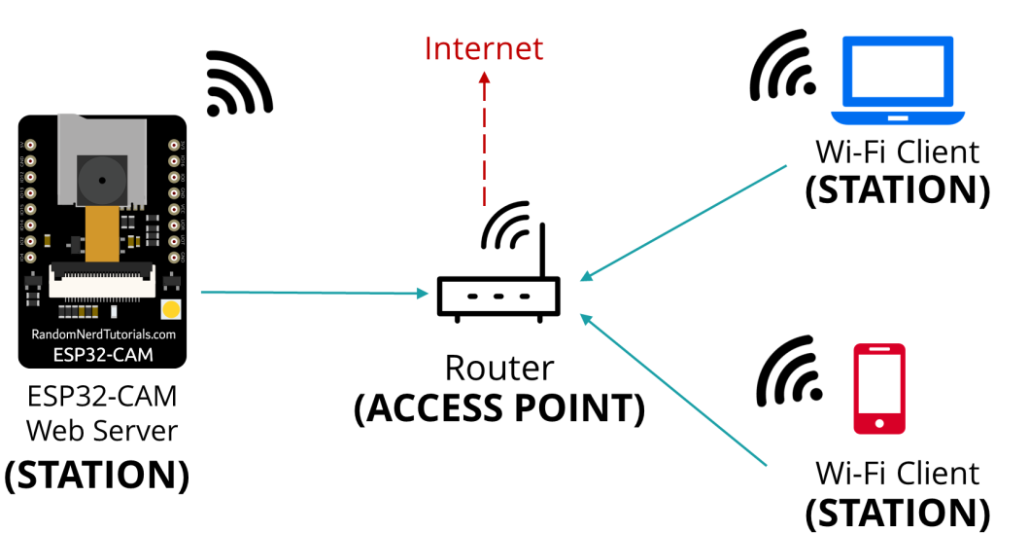
\includegraphics[width=0.5\textwidth]{./images/Chapter3/RouterAsAccessPoint}	
	\caption[نقطه دسترسی و مُد ایستگاهی]{نحوه ارتباط اجزای شبکه \cite{Network}}
	\label{}
\end{figure}
\noindent
\unskip

\subsubsection{شبه‌کد و تشریح جزئیات برنامه}
\label{تشریح اتصال دوربین}
در ادامه، به‌طور دقیق‌تر، فرآیند اتصال ماژول به مودم با استفاده از برنامه نوشته شده در محیط آردوینو را تشریح خواهیم کرد. سپس نحوه استفاده از کتابخانه‌های ارتباط بیسیم برای اتصال به شبکه و اخذ آدرس پروتکل اینترنت \lr{(IP)} به‌عنوان یک مشخصه‌ی مهم برای دستگاه خواهد آمد.
%در اینجا، تعریف و پیاده‌سازی یک مسیر (Route) در فایل apphttpd.cpp برای دریافت درخواست‌های ارسالی از دستگاه تصویربردار انجام می‌پذیرد. سپس توضیح مراحل پردازش درخواست و ارسال پاسخ به دستگاه از طریق این مسیر را ارائه خواهیم داد.%

\section*{}
\begin{latin}
	\lstinputlisting[style=python_style]{code/Pseudocodes/NetworkPseudocode.py}
\end{latin}
در ابتدا به نحوه تنظیم پارامترهای شبکه اعم از نام شبکه \lr{(SSID)} و رمز عبور \lr{(Password)} اشاره می‌کنیم. 
نخست باید مدل دوربین با توجه به ماژول مورد استفاده در برنامه تعریف می‌شود. در این بین دوربین \lr{OV2640} در دسته \lr{AI THINKER} قرار می‌گیرد. سپس نام شبکه و رمزعبور مودم مورد استفاده را در برنامه قرار داده و به تنظیم پارامتر های مهمی در بخش \lr{Setup} در محیط آردوینو پرداخته می‌شود.

%\begin{figure}[h]
%	\centering
%	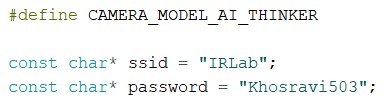
\includegraphics[width=0.3\textwidth]{./images/Chapter3/SSIDPass}	
%	\caption{}
%	\label{}
%\end{figure}
نخست مشخصه \lr{Buad rate} را که بیانگر تعداد تغییرات در سطح سیگنال در یک ثانیه است، برابر 115200 قرار داده شده و سپس پارامترهای تصویر اعم از اندازه تصویر
\noindent\unskip\LTRfootnote{Frame size}،
کیفیت تصویر
\lr{(Jpeg quality)} 
\noindent\unskip\LTRfootnote{Jpeg quality}
و... تنظیم گردید. 

\section*{}
\begin{latin}
	\lstinputlisting[style = cplus_style]{code/CameraWebServer/CameraWebServer.ino}
\end{latin}

در ادامه پیکربندی تعیین شده برای دوربین بررسی گردیده و در صورت عدم وجود خطا در پیکربندی اتصال به روتر شروع می‌گردد. همانطور که در قطعه کد زیر مشخص است با قرار دادن دستورات چاپ در خطوط مختلف برنامه از اتصال کامل ماژول به روتر اطمینان حاصل می‌گردد.
\section*{}
\begin{latin}
	\lstinputlisting[style = cplus_style]{code/CameraWebServer/CameraBegin.ino}
\end{latin}


درانتها نیز آدرس محلی
\noindent\unskip\LTRfootnote{LocalIP}
که روتر به ماژول اختصال می‌دهد، در بخش سریال مانیتور
\noindent\unskip\LTRfootnote{Serial Monitor}
آردوینو چاپ می‌گردد.
%نتیجه این اتصال در شکل س قابل مشاهده است.
\newpage
\subsection{\lr{Handlers}}
\subsubsection{نحوه کارکرد سرور و نقش هندلر‌ها}
در سامانه‌های وب، ارتباط و تبادل اطلاعات بین دستگاه‌ها و سرور
\noindent\unskip\LTRfootnote{Server}
از طریق ارسال درخواست‌
\noindent\unskip\LTRfootnote{Request}
و دریافت پاسخ‌
\noindent\unskip\LTRfootnote{Respond}
به‌وسیله پروتکل های \lr{HTTP} و \lr{HTTPS} و...‌صورت می‌گیرد. وقتی که یک دستگاه یا مرورگر اینترنتی درخواستی به سرور ارسال می‌کند، این درخواست اطلاعاتی از قبیل نوع عملیات  (\lr{DELETE} ،\lr{PUT} ، \lr{POST} ، \lr{GET} و...) و آدرس مورد نظر(\lr{URL})
\noindent\unskip\LTRfootnote{Uniform Resource Locator}
را شامل می‌شود. سرور در این زمان تجزیه و تحلیل درخواست را انجام می‌دهد و با توجه به محتوا و ماهیت درخواست، یک منطق مناسب را فعال می‌سازد.این عملیات‌ها ممکن است شامل دسترسی به پایگاه داده، پردازش اطلاعات، تولید پاسخ‌های مناسب و دیگر عملیات باشند.

در اینجا نقش هندلر
\noindent\unskip\LTRfootnote{Handler}
ها به عنوان یکی از اجزای اصلی سیستم به چشم می‌خورد.هندلرها مسئول پردازش درخواست‌ها و انجام عملیات‌های مختلف میان سرور و دستگاه‌ها هستند. هندلرها اطلاعات درخواست را تجزیه و تحلیل می‌کنند و بر اساس آن‌ها عملیات‌های مورد نیاز را انجام می‌دهند. به عبارت دیگر می‌توان گفت که هندلرها، ارتباط بین دستگاه‌ها و سرور را به صورت منظم و سازماندهی شده‌ای صورت داده و در نتیجه به بهبود عملکرد و کارایی سامانه کمک می‌کند. 

\subsubsection{شبه‌کد و تشریح جزئیات برنامه }
در زیر شبه‌کد
\noindent\unskip\LTRfootnote{Pseudo code}
این بخش مختصرا قراره داده شده و پس از آن به تشریح کامل‌تر آن پرداخته خواهد شد.

\section*{}
\begin{latin}
	\lstinputlisting[style=python_style]{code/Pseudocodes/HandlerPseudocode.py}
\end{latin}

در قطعه برنامه زیر چند هندلر برای مُد‌های مختلف احتمالی تعریف شده‌است. برخی از آنها برای ماژول
\lr{ESP32-CAM}
از پیش تعریف شده‌اند. مهمترین هندلری که با هدف ارسال و مانیتورینگ اطلاعات بین سرور و ماژول و به طبع آن برد
\lr{STM32}
پیاده‌سازی شد،
\lr{current\_color\_uri}
نام دارد. برای این هندلر مقدار
\lr{uri}
که بیانگر مسیر
\noindent\unskip\LTRfootnote{Path}
در آدرس است،
\lr{/currentColor}
تعریف شد. تابع هندلر آن در ادامه بطور کامل‌تر تعریف شده است.
هدف از تعریف این هندلر
\label{PurposeOfOurHandler}
آن است که درخواست ارسال شده به سرور که حاوی اطلاعاتی اعم از رنگ مانع تشخیص داده شده توسط ربات، فاصله ربات تا مانع و... است را دریافت کرده و این اطلاعات از طریق ارتباط
\lr{USART}
, بصورت برخط و با کمترین تاخیر به برد
\lr{STM32}
فرستاده شود.



\section*{}
\begin{latin}
	\lstinputlisting[style = cplus_style]{code/CameraWebServer/defineHandlers.cpp}
\end{latin}

در ادامه چند کانفیگ برای دوربین تنظیم شده که به دلیل طولانی بودن در بخش زیر ذکر نشده‌اند. سپس با بررسی یک شرط، در صورت ارسال موفقیت‌آمیز درخواست از طرف سیستم، تمامی هندلر‌ها چک می‌شوند تا در صورت نیاز پاسخ مناسب را به آن درخواست برگردانند.

\section*{}
\begin{latin}
	\lstinputlisting[style = cplus_style]{code/CameraWebServer/HTTPRequestSendOrNot.cpp}
\end{latin}

همانطور که در
\ref{PurposeOfOurHandler}
ذکر شد، می‌بایست هندلر مورد نظر طوری تعریف شود تا اطلاعات مدنظر به بهترین شکل مدیریت شود.
به همین جهت برای ارسال اطلاعات از
\lr{Query String}
%کوئری استرینگ
%\noindent\unskip\LTRfootnote{Query String}
استفاده شده است.

\subsubsection{کوئری استرینگ}

‏گاهی‌اوقات لازم است که وب‌سایت از وضعیت
\noindent\unskip\LTRfootnote{State}
ما مطلع باشد و بتواند در همان لحظه، مسیری را طی کند. مثلا زمانی که قصد داریم یک فرم چند صفحه‌ای را پر کنیم، سرور باید مطلع باشد که ما در صفحه پیش چه کاری انجام دادیم و یا به عنوان مثالی دیگر می‌توان به مراحل یک خرید اینترنتی (اضافه کردن کالاها به سبد خرید، پرداخت آنلاین و...) اشاره کرد.

پروتکل
\lr{HTTP}
امکان نگهداری وضعیت را ندارد. پس مکانیزم‌های دیگری به‌وجود آمدند تا بتوانند این کار را انجام دهند. از جمله‌ی این مکانیزم‌ها می‌توان به نگهداری وضعیت سمت سرور با استفاده از 
\lr{Session}
و یا نگهداری وضعیت سمت کاربر
\noindent\unskip\LTRfootnote{Client}
با استفاده از کوکی
\noindent\unskip\LTRfootnote{Cookie}
اشاره کرد.
مکانیزم دیگری برای نگهداری وضعیت و انتقال اطلاعات بين صفحات وجود دارد. در این مکانیزم همراه با درخواست‌ها، وضعیت قبلی را نیز از طریق
\lr{URL}
جدیدی که فراخوانی می‌شود، به سرور داده می‌شود. به این روش کوئری استرینگ گفته می‌شود.
کوئری استرینگ هر مقداریست که بعد از علامت سوال $(“?”)$ در انتهای
\lr{URL}
قرار می‌گیرد که می‌تواند یک یا تعداد بیشتری پارامتر باشد.
\noindent
ساختار کوئری استرینگ را در شکل زیر مشاهده می‌کنید:

\begin{figure}[h]
	\centering
	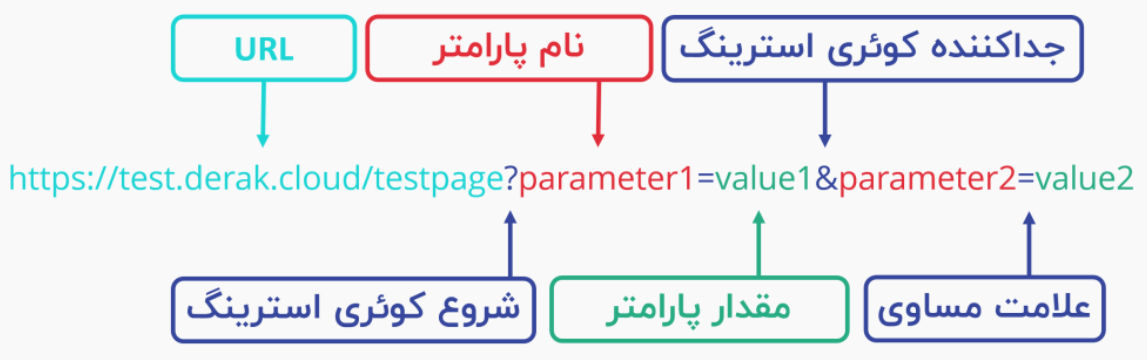
\includegraphics[width=0.7\textwidth]{./images/Chapter3/QueryStringStructure}	
	\caption[ساختار کوئری استرینگ]{ساختار کوئری استرینگ \cite{QueryString}}
	\label{ساختار کوئری}
\end{figure}
\noindent
\unskip

همانطور که در شکل
\ref{ساختار کوئری}
مشخص است آدرس های شامل کوئری استرینگ دارای بخش‌های مختلفی می‌باشند.
\begin{itemize}
	\item 
	\lr{URL} : این بخش شامل دامنه مورد نظر است. همچنین از اجزای دیگر آن می‌توان به پروتکل، زیردامنه و مسیر اشاره کرد که در نهایت یک آدرس را تشکیل می‌دهد.
	\item
	$?$ : ابتدای کوئری استرینگ با این علامت شروع می‌شود و پس از آدرس قرار می‌گیرد.
	\item
	نام پارامتر: در کوئری استرینگ پارامترهای مختلف را می‌بینیم که هر پارامتر یک نام
	\noindent\unskip\LTRfootnote{Key}
	و یک مقدار
	\noindent\unskip\LTRfootnote{Value}
	دارد. پس از علامت سوال، نام اولین پارامتر دیده می‌شود.
	\item
	$=$ : برای تعیین مقدار یک پارامتر از این علامت استفاده می‌شود و پس از نام پارامتر قرار می‌گیرد.
	\item
	\lr{\&} : برای جداسازی پارامتر‌های مختلف از این علامت استفاده می‌شود. این علامت بین مقدار پارامتر قبلی و نام پارامتر بعدی قرار می‌گیرد.
\end{itemize}
%\newpage
استفاده از این روش مزایا و معایب متفاوتی دارد که در ذیل مختصرا به آن‌ها اشاره شده‌است.
\cite{QueryString}
مزایا:
\begin{itemize}
	
	\item
	استفاده ساده
	\item
	سریع‌ترین روش انتقال اطلاعات بين صفحات
	\item
	عدم تحميل عمليات اضافه به سرويس‌دهنده و در نتیجه هزینه‌ی کم
\end{itemize}

معایب:
\begin{itemize}
	
	\item
	اطلاعات، محدود به رشته‌های ساده است (فقط کاراکترهای مجاز)
	\item
	اطلاعات همواره به عنوان يک رشته بازيابی می‌شوند و در صورت نياز باید آن‌ها را به نوع داده مورد نظر تبديل كرد.
	\item
	اطلاعات توسط همه قابل مشاهده‌است. برای مواردی که لازم است اطلاعاتی به‌طور مخفی از يک صفحه به صفحه ديگر ارسال و يا بر روی آن حساسيت خاصی از نظر امنيتی وجود دارد، قابل استفاده نیست.
	\item
	كاربران می توانند محتويات کوئری استرینگ را تغيير داده و در بعضی موارد باعث ایجاد مشکل شوند.
	\item
	تعداد زيادی از مرورگرها برای طول یک
	\lr{URL}
	محدودیت دارند. بنابراين، نمی‌توان حجم بالایی از اطلاعات را در کوئری استرینگ ذخيره كرد.
\end{itemize}
\newpage
\subsubsection{تابع هندلر}
در زیر شبه‌کد این بخش مختصرا قرار داده شده و پس از آن به تشریح کامل‌تر آن پرداخته خواهد شد.
\section*{}
\begin{latin}
	\lstinputlisting[style=python_style]{code/Pseudocodes/CurrentColorPseudocode.py}
\end{latin}

در برنامه زیر ابتدا یک بافر
\noindent\unskip\LTRfootnote{Buffer}
با مقدار زیاد انتخاب شده و سپس اگر یک درخواست از نوع
\lr{GET}
که دارای کوئری استرینگ باشد برای سرور ارسال شده باشد، آنگاه نام پارامتر آن بررسی می‌شود و اگر برابر
\lr{color}
بوده باشد، مقدار آن پارامتر به عنوان داده معتبر درون بافر ریخته می‌شود. سپس دیتای داخل بافر را از طریق ارتباط
\lr{UART}
برای
\lr{STM32}
ارسال و سپس داده داخل بافر برای درخواست بعدی خالی می‌شود. 
\section*{}
\begin{latin}
	\lstinputlisting[style = cplus_style]{code/CameraWebServer/ColorHandlers.cpp}
\end{latin}

\subsection{ارتباط \lr{USART}}
انتقال اطلاعات را می توان به دو روش کلی موازی و سریال انجام داد.در روش انتقال موازی چند بیت اطلاعات به وسیله چند خط انتقال می‌یابد و در روش انتقال سریال در هر لحظه فقط یک بیت ارسال می‌شود. در مقایسه بین این دو روش می‌توان گفت که در روش انتقال موازی به علت انتقال چند بیت اطلاعات در یک لحظه، سرعت آن نسبت به سریال که در یک لحظه فقط یک بیت را انتقال می‌دهد بیشتر است. همچنین برای فواصل طولانی بکار بردن روش انتقال موازی به علت ازدیاد سیم‌های ارتباطی، دارای هزینه بالا می‌باشد؛ بنابراین در فواصل طولانی انتقال به روش سریال مناسب تر است.

\textbf{فرستنده و گیرنده سریال همزمان و غیر همزمان جهانی} یا \lr{USART } یک ارتباط از نوع انتقال سریال می باشد که امکان ارتباط دوطرفه کامل را می‌دهد و برای ارتباط بین دو دستگاه مفید می‌باشد.
در حالتی که هیچ ارسال و دریافتی انجام نمی‌شود یا اصطلاحاً خط انتقال در حالت بیکار \lr{(Idle)} قرار دارد، سطح ولتاژ مربوط به یک منطقی بر روی خط ارسال قرار می‌گیرد. تغییر وضعیت از یک به صفر منطقی به معنی شروع ارسال است و گیرنده آماده دریافت اطلاعات می‌شود. این صفر شدن به مدت یک بیت باید طول بکشد و به آن "بیت شروع" گفته می‌شود. بعد از آن یک بایت داده به ترتیب از بیت کم ارزش \lr{(LSB)} به بیت پرارزش \lr{(MSB)} ارسال می‌شود. در نهایت یک بیت برای آزمایش شدن درستی داده ارسال شده، روی خط ارسال قرار می‌گیرد که بیت "بیت توازن" نام دارد.

نرخ انتقال‌های که به صورت قراردادی بین فرستنده و گیرنده در یک ارتباط سریال، مشخص می‌شود مقادیر خاصی می‌توانند داشته باشند که مقدارهای ۴۸۰۰، ۱۹۲۰۰ ،۹۶۰۰، ۳۸۴۰۰، ۵۷۶۰۰، ۱۱۵۲۰۰ (بیت بر ثانیه) از معمول‌ترین این مقادیرند. در انجام آزمایش های عملی بر روی ربات از نرخ ۱۱۵۲۰۰ بیت بر ثانیه استفاده شده است.
%مثلاً نرخ انتقال ۹۶۰۰ به این معنی است که در هر ثانیه ۹۶۰۰ بیت منتقل می‌شود. پس هر بیت در فاصلهٔ زمانی ۱۰۴٫۱۶۶ میکروثانیه باید منتقل شود و در تمام این مدت مقدار خود را حفظ کند تا گیرنده نمونه برداری مناسبی انجام دهد.%


\section{اتصال دو برد به یکدیگر}


در این بخش، روش اتصال دو برد \lr{ESP32 CAM } و \lr{STM32f103c8t6} به یکدیگر از طریق رابط \lr{USART} تشریح خواهد شد. رابط \lr{USART} یک رابط سریالی است که امکان انتقال داده‌ها بین دو دستگاه را فراهم می‌کند. این رابط اغلب برای ارتباط میان میکروکنترلرها و ماژول‌ها استفاده می‌شود. استفاده از این روش برای ارتباط بین دو دستگاه از اهمیت ویژه‌ای در تبادل اطلاعات در پروژه‌های الکترونیکی و رباتیک برخوردار است و تجربه کار با رابط‌های سریالی را به ارمغان می‌آورد.

ابتدا به تعیین پایه‌های \lr{RX} و \lr{TX} در هر یک از دو برد پرداخته و تنظیمات مورد نیاز در هر دستگاه برای فعال‌سازی رابط \lr{USART} انجام می‌شود. بدین منظور همانطور که در شکل 
\ref{اتصال دو برد}
مشخص است پایه
\lr{UOR}
از ماژول
\lr{ESP32-CAM}
که برای دریافت اطلاعات تعبیه شده‌است، به پایه
\lr{PA9}
از برد
\lr{STM32}
که برای ارسال اطلاعات تعبیه شده‌است، متصل می‌باشد. همچنین پایه
\lr{UOT}
از ماژول
\lr{ESP32-CAM}
که برای ارسال اطلاعات تعبیه شده‌است، به پایه
\lr{PA10}
از برد
\lr{STM32}
که برای دریافت اطلاعات تعبیه شده‌است، متصل می‌باشد. برای تامین انرژی مدار نیز پایه زمین هر دو مدار و منبع تغذیه یکسان شده و ولتاژ منبع تغذیه بر روی 5 ولت تنظیم خواهد شد.

\vspace{1cm}
\begin{figure}[h]
	\centering
	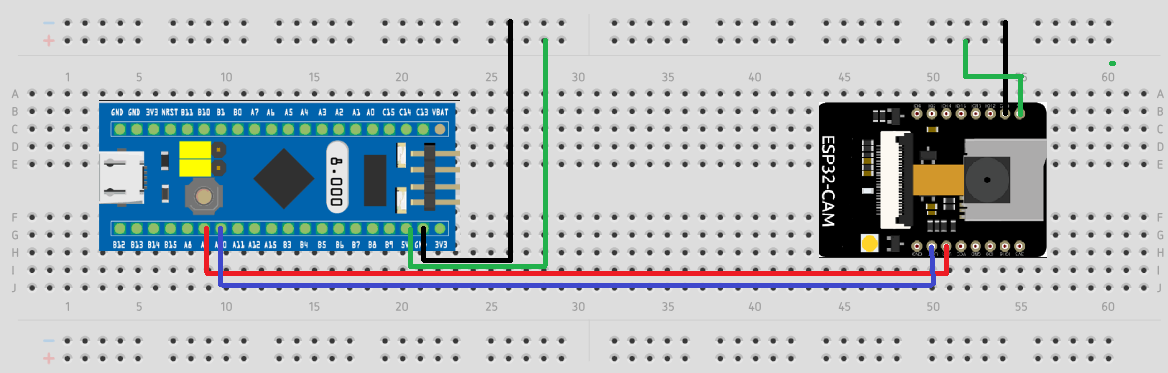
\includegraphics[width=1\textwidth]{./images/Chapter3/TwoBoardConnection}	
	\caption{نحوه اتصال دو برد  به یکدیگر}
	\label{اتصال دو برد}
\end{figure}
\newpage
\section{جمع‌بندی}

در این فصل با توجه به اهمیت انتقال و مدیریت داده بین خود و ربات به طراحی یک سرور و نحوه ارتباط بخش‌های مختلف الکتریکی با یکدیگر پرداخته شد. بدین منظور از روشی با نام کوئری استرینگ استفاده شد. در این روش داده مورد نظر را در دو بخش (نام پارامتر، مقدار پارامتر) منتقل کرده و در سمت دیگر توسط همین دو معیار قابل شناسایی می‌باشند. همچنین برای پاسخ مناسب به درخواست‌های ارسال شونده به سمت سرور توسط توابعی که بطور معمول آن‌ها را هندلر می‌نامند، چند حالت مختلف درخواست و پاسخ طراحی گردید.

\chapter{سخت افزار الکترونیکی ربات}

\section{مقدمه}

\section{پردازنده \lr{ARM} سری \lr{f101c8t6}}

شاید واژه
\lr{ARM}
\noindent\unskip\LTRfootnote{Advanced RISC Machine}
برایتان آشنا باشد.
\lr{ARM}
نوعی معماری برای ساخت انواع پردازنده‌های 32 و 64 بیتی است. از دلایل محبوبیت و استفاده از پردازنده‌هایی با این معماری در انواع سیستم‌های نهفته
\noindent\unskip\LTRfootnote{Embedded Systems}،
می‌توان به قیمت مناسب، سرعت بالاتر، توان مصرفی پایین و... اشاره کرد. عدد بعد از این حروف نشانگر تعداد خطوط اجرایی
\noindent\unskip\LTRfootnote{performance lines}
پردازنده می‌باشد. یکی از شرکت‌هایی که این معماری را برای ساخت پردازنده های خود انتخاب می‌کند، شرکت
\lr{ST}
می‌باشد. میکروکنترلرهای این شرکت تحت عنوان
\lr{STM}
بعلت تنوع بالا و ارائه کتابخانه های برنامه‌نویسی کاربردی، بسیار مشهور شده‌اند.

\begin{figure}[H]
	\centering
	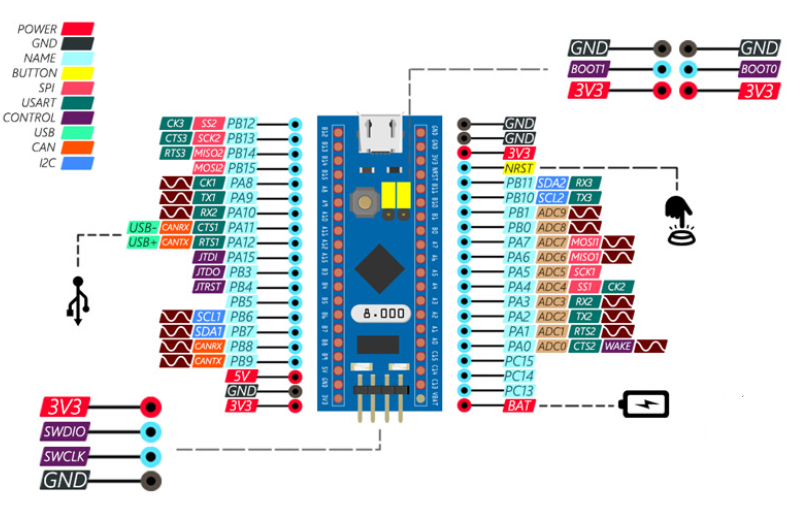
\includegraphics[width=1\textwidth]{./images/Chapter4/STM32Pinout}
	\caption[]{ \cite{STM32F101}}
	\label{پایه‌های آرم}
\end{figure}


\section{ماژول \lr{ESP32-CAM}}

ماژول
\lr{ESP32-CAM}
یک ماژول کامل است که برای بسیاری از کاربردهای صنعتی و اینترنت اشیاء استفاده می‌شود. همچنین دارای قابلیت‌های متعددی اعم از انواع ارتباطات، ذخیره‌سازی اطلاعات و... بوده و دارای مشخصات فنی زیر می‌باشد:
% \cite{ESP32details}
\begin{itemize}
	\item 
	ارتباطات: بلوتوث 4.2 \lr{BLE} به همراه \lr{Wifi 802.11b}. که از بارگذاری تصویر از طریق \lr{WiFi} پشتیبانی می کند.
	\item
	اتصالات: \lr{UART} ، \lr{SPI} ، \lr{I2C}، و \lr{PWM} و دارای 9 پایه \lr{GPIO} است.
	\item
	فرکانس ساعت: تا 160 مگاهرتز
	\item
	قدرت محاسباتی میکروکنترلر: حداکثر 600 \lr{DMIPS}.
	\item
	حافظه: 520 کیلوبایت \lr{SRAM}، چهار مگابایت حافظه کارت \lr{PSRAM + SD}
	\item
	دوربین: از دوربین های \lr{OV2640} پشتیبانی می‌کند که دارای 2 مگاپیکسل روی سنسور با اندازه آرایه  1622 × 1200\lr{UXGA} پیکسل هستند.
\end{itemize}



برای اتصال این ماژول به کامپیوتر و برنامه‌ریزی
\noindent\unskip\LTRfootnote{Programming}
آن می‌توان از دو روش استفاده کرد:

1-استفاده از یک مبدل \lr{USB} به سریال مانند

2-استفاده از یک برد دیگر مانند آردوینو
\noindent\unskip
\noindent\unskip\RTLfootnote{برای برنامه‌ریزی از طریق ارتباطاتی همچون \lr{UART}}


\begin{figure}[H]
	\centering
	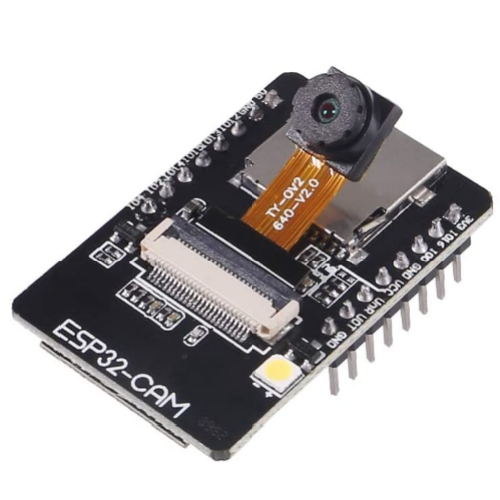
\includegraphics[width=0.4\textwidth]{./images/Chapter4/ESP32CAM}
	\caption[ماژول \lr{ESP32CAM}]{ماژول \lr{ESP32CAM} \cite{ESP32CAM}}
	\label{ماژول ای اس پی}
\end{figure}

نکته بسیار مهم اینکه برای برنامه ریزی شدن این ماژول باید حتما حین برنامه ریزی دو پایه ی \lr{Io0} و\lr{GND} به یکدیگر متصل باشند. همچنین پس از تکمیل برنامه ریزی باید اتصال این دو پایه را قطع کرد.\\ 

\section{دوربین \lr{OV2640}}
دوربین \lr{OV2640} یک سنسور تصویر \lr{CMOS} با رزولوشن بالا است که توسط شرکت \lr{OmniVision} تولید می‌شود.این دوربین به ویژه برای برنامه‌هایی مناسب است که نیاز به تصاویر با کیفیت بالا و ویژگی‌های پیشرفته دارند. از آنجا که این دوربین بسیار محبوب و پرطرفدار است، در بسیاری از پروژه‌های الکترونیک و رباتیک استفاده می‌شود، از جمله پروژه‌هایی که به آن اشاره کردید، یعنی ربات عنکبوتی چهار پا.


\begin{figure}[h]
	\centering
	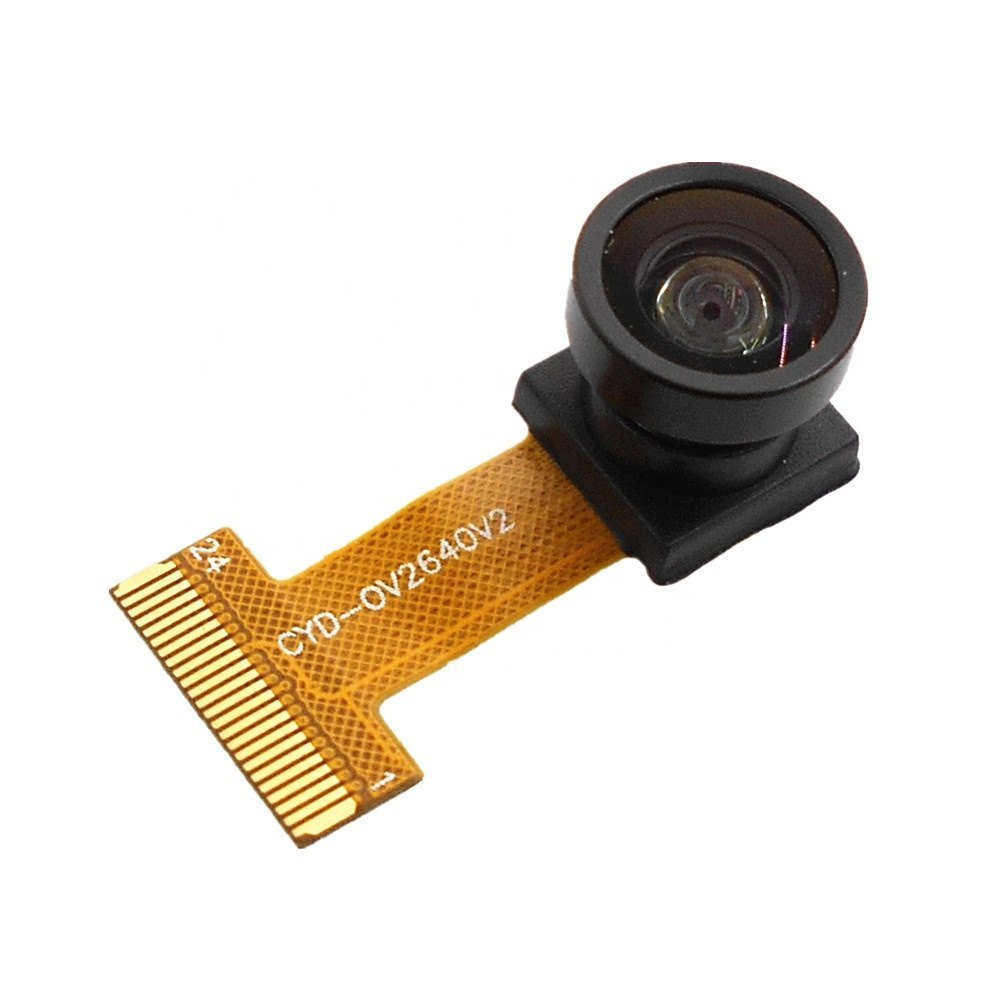
\includegraphics[width=0.4\textwidth]{./images/Chapter4/OV2640}
	\caption[دوربین \lr{OV2640}]{دوربین \lr{OV2640} \cite{OV2640}}
	\label{عکس دوربین}
\end{figure}

ویژگی‌های کلیدی دوربین \lr{OV2640} عبارت‌اند از:
\begin{itemize}
	\item
	رزولوشن بالا: دوربین \lr{OV2640} قابلیت ثبت تصاویر با رزولوشن بالا را دارد. این دوربین قابلیت ثبت تصاویر با رزولوشن حداکثر 2 مگاپیکسل ($1200 \times 1600$) را دارد.
	
	\item
	فرمت تصویری متنوع: این دوربین از فرمت‌های مختلف تصویری مانند \lr{RGB} ، \lr{YUV} ، \lr{JPEG} و \lr{Raw}  پشتیبانی می‌کند که این امر به کاربر امکان انتخاب فرمتی مناسب با توجه به نیازهای پروژه را می‌دهد.
	\item
	تمرکز اتوماتیک \lr{(Auto-Focus)}: دوربین \lr{OV2640} دارای ویژگی تمرکز اتوماتیک بر روی تصاویر است که بهترین تنظیمات فوکوس را برای صحنه‌ها و شرایط مختلف فراهم می‌کند.
	\item
	تنظیمات تصویری: این دوربین اجازه تنظیمات مختلف تصویری مانند شدت روشنایی \lr{(Exposure)}, توازن رنگ \lr{(White Balance)}, کنتراست \lr{(Contrast)} و... را به کاربر می‌دهد.
	\item
	حالت تصویربرداری پیوسته \lr{(Continuous Shooting)}: با امکان ثبت تصاویر به صورت پیوسته، دوربین \lr{OV2640} مناسب برای برنامه‌هایی است که نیاز به ثبت تصاویر متوالی دارند.
	\item
	حالت‌های مختلف عکسبرداری: این دوربین از حالت‌های مختلف عکسبرداری مانند \lr{Single Capture}، \lr{Raw Capture} و \lr{JPEG Capture} پشتیبانی می‌کند.
	\item
	پشتیبانی از ارتباطات: دوربین \lr{OV2640} از ارتباطات مختلف مانند \lr{I2C} ، \lr{UART} و \lr{SPI} پشتیبانی می‌کند که این امر ارتباط آسان با میکروکنترلرها و ماژول‌های دیگر را ممکن می‌سازد.
	\item
	کاربرد وسیع: دوربین \lr{OV2640} به عنوان یک ماژول کوچک و قابل حمل، در بسیاری از پروژه‌های رباتیک، دوربین‌های مدار بسته، دوربین‌های امنیتی، دستگاه‌های پزشکی و سایر برنامه‌های صنعتی و مصرفی مورد استفاده قرار می‌گیرد.
\end{itemize}
با توجه به ویژگی‌های برتر دوربین \lr{OV2640}، می‌توان آن را به عنوان یک گزینه مناسب برای پروژه‌های شما در زمینه‌های رباتیک و دید کامپیوتری در نظر گرفت.

\section{سروموتور}
سروموتورها از جمله اجزاء اساسی در رباتیک و به‌ویژه در ربات‌های چهارپا مورد استفاده قرار می‌گیرند. این اجزا جهت کنترل و حرکت اندام‌ها و پاهای ربات به کار می‌روند. سروموتورها معمولاً دارای یک شفت قابل چرخش هستند که از طریق یک سیگنال کنترلی به جلو و عقب حرکت می‌کنند. سروموتورها به دلیل دقت، سرعت و کاربرد‌های متعددشان، بخش مهمی از طراحی و ساخت ربات‌های چهارپا را تشکیل می‌دهند.

در ربات‌های چهارپا، سروموتورها به‌عنوان موتورهای اصلی برای حرکت پاها و اندام‌ها عمل می‌کنند. این سروموتورها معمولاً دقیق و قابل کنترل با سرعت متغیر هستند، که این ویژگی‌ها امکان جابه‌جایی دقیق و پیچیده را فراهم می‌کنند. سروموتورها معمولاً با استفاده از میکروکنترلرها به راحتی کنترل می‌شوند. این اجزا به تنهایی یا به صورت گروهی در ربات‌های چهارپا استفاده می‌شوند تا حرکت و موقعیت دقیق در سیستم رباتیک تضمین شود.

\begin{figure}[h]
	\centering
	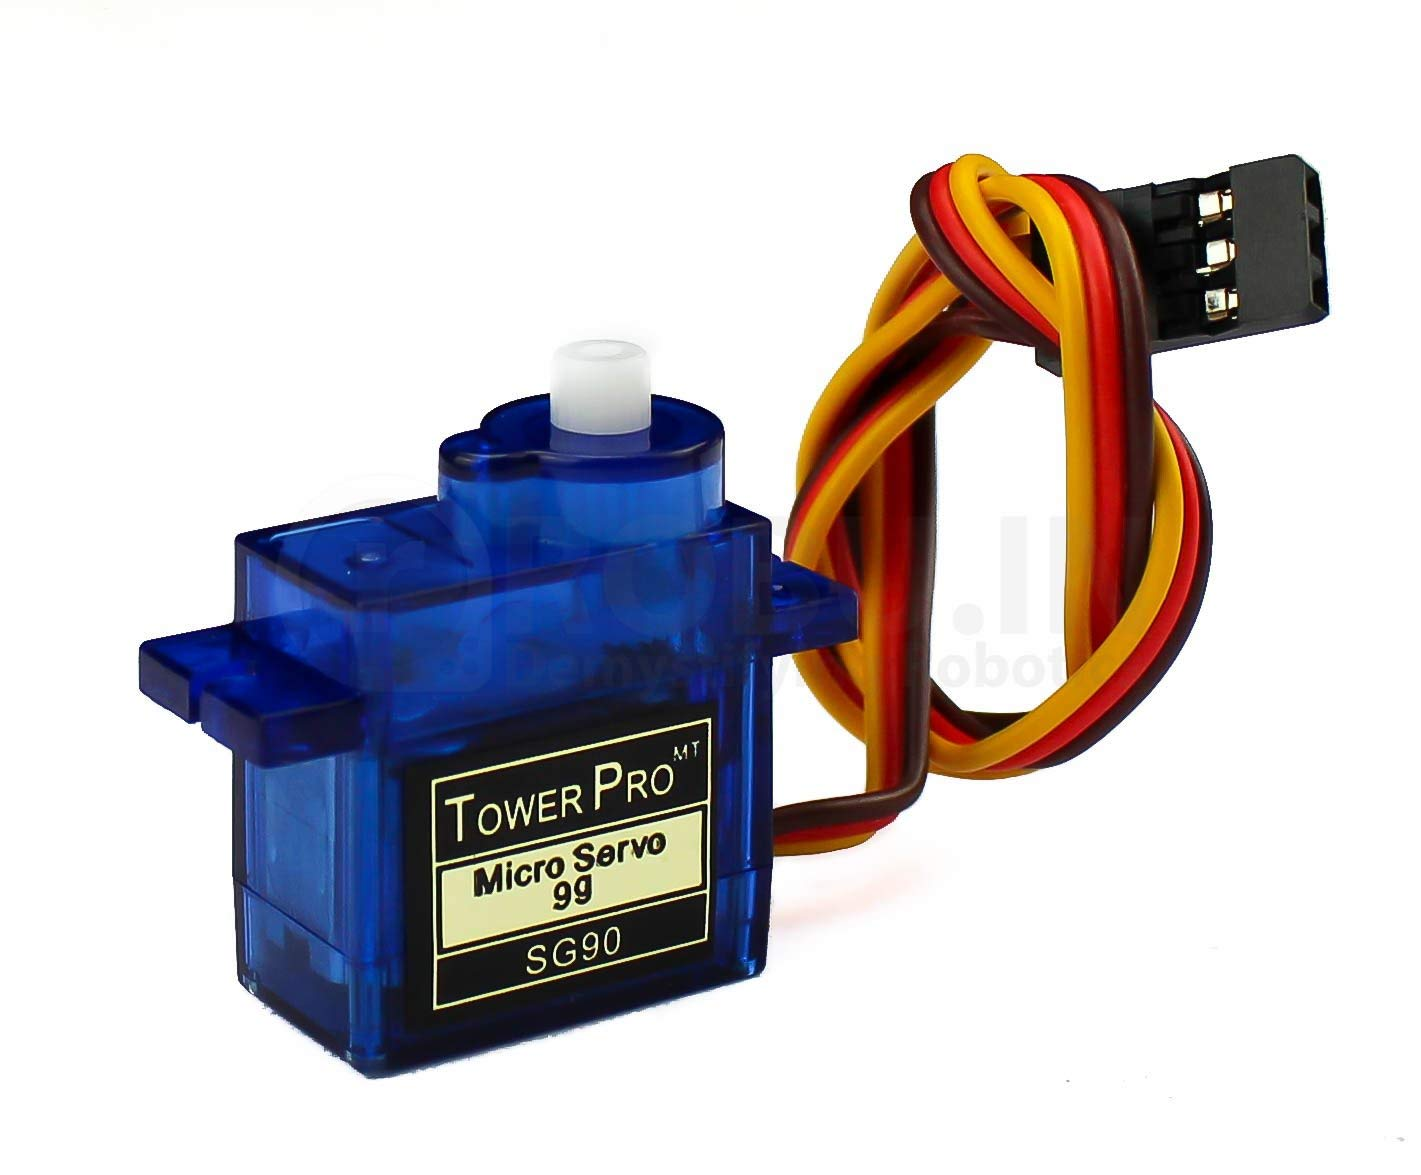
\includegraphics[width=0.4\textwidth]{./images/Chapter4/ServoMotor}
	\caption[سروموتور \lr{SG90}]{سروموتور \lr{SG90} \cite{ServoMotor}}
	\label{سروموتور}
\end{figure}

\subsection{روش \lr{PWM}}
\subsubsection{مدولاسیون چیست؟}
احتمالا عبارت‌های \lr{AM} و \lr{FM} را روی وسایل الکتریکی مانند رادیو و... مشاهده کرده اید.عبارت \lr{AM}، مخفف \lr{Amplitude Modulation} به‌معنی مدولاسیون دامنه و عبارت \lr{FM} مخفف مدولاسیون فاز است. مدولاسیون دامنه، راهی برای ارسال یک سیگنال روی یک حامل است.مدولاسیون اساساً یک راه برای رمزگذاری یک سیگنال بر روی سیگنال حامل است.

به عبارت دیگر مدولاسیون سوار کردن سیگنال مورد نظر بر روی یک سیگنال دیگر است. اینکار به‌منظور افزایش برد سیگنال و بهره‌وری انتقال انجام می‌شود. به‌طور کلی، فرایند گنجاندن سیگنال حاوی اطلاعات در سیگنالی دیگر را مدولاسیون می‌نامند.

\subsubsection{مدولاسیون پهنای پالس}
مدولاسیون پهنای پالس یا \lr{PWM} ، نوعی سیگنال است که می‌توان آن را توسط یک مدار مجتمع دیجیتال مانند میکروکنترلر تولید کرد. این سیگنال تولیدی یک قطار پالس بوده و یک شکل‌موج مربعی را تشکیل می‌دهند. به عبارتی در هر زمان مشخص، سیگنال تنها می‌تواند دو وضعیت بالا \lr{(High)} که معادل 1 دیجیتالی و یا پایین \lr{(Low)} که معادل صفر دیجیتالی است را به خود اختصاص دهد.

مدت‌زمانی که سیگنال در وضعیت \lr{High} قرار دارد، «زمان روشن» \lr{(On Time)}و مدت‌زمانی که سیگنال در وضعیت \lr{Low} است، «زمان خاموش» \lr{(Off Time)} نامیده می‌شود.

\section{تجهیزات مکانیکی}

\subsection{سایر قطعات متصل کننده}
پین هدر ها و ...

\section{جمع بندی}
همانطور که در بخش های این فصل بررسی شد، تمامی سخت‌افزار های استفاده شده در پروژه اعم از الکترونیکی و یا مکانیکی و یا سایر تجهیزات همگی با در نظر گرفتن کاربری تا حدامکان بصورت اقتصادی انتخاب شده و همچنین قابل دسترس در بازار ایران می‌باشند.
از سوی دیگر داشتن شناخت کافی از جزئیات و اطلاعات فنی هریک از سخت‌افزار‌ها منجر به انتخاب  قطعات معرفی شده در کمترین زمان ممکن انجامید.


\chapter{جمع‌بندي و نتيجه‌گيري و پیشنهادات}
%%%%%%%%%%%%%%%%%%%%%%%%%%%%%%%%%%%%%%%%%%%
در پايان گزارش‌هاي علمي و فني لازم است كه جمع‌بندي يا نتيجه‌گيري نهايي ارائه شود. در اين موارد مي‌توان آخرين فصل پایان نامه كه پیش از مراجع قرار مي‌گيرد را به اين امر اختصاص داد.
\section{پیشنهادات}
در این بخش پیشنهاداتی که محقق جهت ادامه تحقیقات دارد ارایه می‌گردد. دقت شود که پیشنهادات باید از  تحقیق انجام شده و نتایج ان حاصل شده باشد و از ذکر جملات کلی باید پرهیز کرد.

%--------------------------------------------------------------------------appendix( مراجع و پیوست ها)
\chapterfont{\vspace*{-2em}\centering\LARGE}%

\appendix
\bibliographystyle{plain-fa}
\bibliography{references}
\chapter*{‌پیوست}
\markboth{پیوست}{}
\addcontentsline{toc}{chapter}{پیوست}
%موضوعات مرتبط با متن گزارش پایان نامه كه در يكی از گروه‌های زير قرار می‌گيرد، در بخش پيوست‌ها آورده شوند:
%\begin{enumerate}
%\item  اثبات های رياضی يا عمليات رياضی طولانی‌.‌
%\item داده و اطلاعات نمونه (های) مورد مطالعه (\lr{Case Study}) چنانچه طولانی باشد‌.‌
%\item نتايج كارهای ديگران چنانچه نياز به تفصيل باشد‌.‌
%\item مجموعه تعاريف متغيرها و پارامترها، چنانچه طولانی بوده و در متن به انجام نرسيده باشد‌.‌
%\end{enumerate}
% براي شماره‌گذاري روابط، جداول و اشكال موجود در پيوست‌ از ساختار متفاوتي نسبت به متن اصلي استفاده مي‌شود كه در زير به‌عنوان نمونه نمايش داده شده‌است. 
% \begin{equation}
	%F=ma
	%\end{equation}
	\section*{کد پایتون \lr{RRT}}
	\textbf{ماژول نوشته شده شامل کلاس‌های استفاده شده در فایل اجرایی :}
	\begin{latin}
		\lstinputlisting[style=python_style]{code/RRTalgorithm/RRTbasePy.py}
	\end{latin}
	
	\textbf{فایل اصلی جهت اجرا :}
	
	\begin{latin}
		\lstinputlisting[style=python_style]{code/RRTalgorithm/RRT.py}
	\end{latin}
	\section{کد \lr{Localization}}
	\textbf{کد مکان‌یابی برای سنجش صحت پارامتر‌های دوربین و ارتباط با ربات}
	\begin{latin}
		\lstinputlisting[style=python_style]{code/Localization/Aruco.py}
	\end{latin}
	

%--------------------------------------------------------------------------dictionary(واژه نامه ها)
%اگر مایل به داشتن صفحه واژه‌نامه نیستید، خط زیر را غیر فعال کنید.
\parindent=0pt
%
\chapter*{واژه‌نامه‌ی فارسی به انگلیسی}
\pagestyle{style9}

\addcontentsline{toc}{chapter}{واژه‌نامه‌ی فارسی به انگلیسی}
%%%%%%
\begin{multicols*}{2}

{\bf آ}
\vspace*{3mm}


\farsiTOenglish{اسکالر}{Scalar}


\vspace*{3mm}
{\bf ب}
\vspace*{3mm}

\farsiTOenglish{بالابر}{Lift}


\vspace*{3mm}
{\bf پ}
%%\vspace*{3mm}

\farsiTOenglish{پایا}{Invariant}



\vspace*{3mm}
{\bf ت}
%%\vspace*{3mm}

\farsiTOenglish{ تناظر }{Correspondence}


\vspace*{3mm}
{\bf ث}
%%\vspace*{3mm}

\farsiTOenglish{ثابت‌ساز}{Stabilizer}

\vspace*{3mm}
{\bf ج}
%%\vspace*{3mm}

\farsiTOenglish{جایگشت}{Permutation}



\vspace*{3mm}
{\bf چ}
%%\vspace*{3mm}


\farsiTOenglish{چند جمله‌ای }{Polynomial}

\vspace*{3mm}
{\bf ح}
%%\vspace*{3mm}

\farsiTOenglish{حاصل‌ضرب دکارتی}{Cartesian product}


\vspace*{3mm}
{\bf خ}
%%\vspace*{3mm}

\farsiTOenglish{خودریختی}{Automorphism}

\vspace*{3mm}
{\bf د}
%%\vspace*{3mm}

\farsiTOenglish{درجه}{Degree}


\vspace*{3mm}
{\bf ر}
%%\vspace*{3mm}


\farsiTOenglish{ریزپردازنده}{microprocessor}


\vspace*{3mm}
{\bf ز}
%%\vspace*{3mm}


\farsiTOenglish{زیرمدول}{Submodule}


\vspace*{3mm}
{\bf س}
%%\vspace*{3mm}

\farsiTOenglish{سرشت}{Character}


\vspace*{3mm}
{\bf ص}
%%\vspace*{3mm}

\farsiTOenglish{صادقانه}{Faithful}

\vspace*{3mm}
{\bf ض}
%%\vspace*{3mm}

\farsiTOenglish{ضرب داخلی}{Inner product}

\vspace*{3mm}
{\bf ط}
%%\vspace*{3mm}


\farsiTOenglish{طوقه}{Loop}


\vspace*{3mm}
{\bf ظ}
%%\vspace*{3mm}


\farsiTOenglish{ظرفیت}{Valency}
 
\vspace*{3mm}
{\bf ع}
%%\vspace*{3mm}


\farsiTOenglish{عدم مجاورت}{Nonadjacency}



\vspace*{3mm}
{\bf ف}
%%\vspace*{3mm}

\farsiTOenglish{فضای برداری}{Vector space}



\vspace*{3mm}
{\bf ک}
%%\vspace*{3mm}

\farsiTOenglish{کاملاً تحویل‌پذیر}{Complete reducibility}


\vspace*{3mm}
{\bf گ}
%%\vspace*{3mm}


\farsiTOenglish{گراف}{Graph}



\vspace*{3mm}
{\bf م}
%%\vspace*{3mm}

\farsiTOenglish{ماتریس جایگشتی}{Permutation matrix }


\vspace*{3mm}
{\bf ن}
%%\vspace*{3mm}

\farsiTOenglish{ناهمبند}{Disconnected}


\vspace*{3mm}
{\bf و}
%%\vspace*{3mm}

\farsiTOenglish{وارون‌پذیر}{Invertible}


\vspace*{3mm}
{\bf ه}
%%\vspace*{3mm}

\farsiTOenglish{همبند}{Connected}



\vspace*{3mm}
{\bf ی}
%%\vspace*{3mm}

\farsiTOenglish{یال}{Edge}




\end{multicols*}%
%%%%%%
\chapter*{ واژه‌نامه‌ی انگلیسی به فارسی}
\pagestyle{style9}
\lhead{\thepage}\rhead{واژه‌نامه‌ی انگلیسی به فارسی}
\addcontentsline{toc}{chapter}{واژه‌نامه‌ی انگلیسی به فارسی}

\LTRmulticolcolumns
\begin{multicols}{2}
{\hfill\bf  \lr{A}}
%%\vspace*{1.5mm}

\englishTOfarsi{Access Point}{نقطه دسترسی}
\englishTOfarsi{Actuator}{عملگر}
\englishTOfarsi{Artificial Potential Field}{میدان پتانسیل مصنوعی}
\englishTOfarsi{Ant Colony Optimization}{بهینه‌سازی کلونی مورچه‌ها}
\englishTOfarsi{Assemble}{سرهم کردن}

\vspace*{3mm}
{\hfill\bf   \lr{B}}
%%\vspace*{1.5mm}

\englishTOfarsi{Base}{تکیه‌گاه}

\vspace*{3mm}
{\hfill\bf   \lr{C}}
%%\vspace*{1.5mm}

\englishTOfarsi{Conventional}{مرسوم}
\englishTOfarsi{Client}{کاربر}
\englishTOfarsi{Cell Decomposition}{تجزیه سلولی}

\vspace*{3mm}
{\hfill\bf   \lr{D}}
%%\vspace*{1.5mm}

\englishTOfarsi{Degree}{درجه}
\englishTOfarsi{Dynamic}{پویا}

\vspace*{3mm}
{\hfill\bf   \lr{E}}
%%\vspace*{1.5mm}

\englishTOfarsi{Edge}{یال}

\vspace*{3mm}
{\hfill\bf   \lr{F}}
%%\vspace*{1.5mm}

\englishTOfarsi{Function}{تابع}

\vspace*{3mm}
{\hfill\bf   \lr{G}}
%%\vspace*{1.5mm}

\englishTOfarsi{Graph}{گراف}

\vspace*{3mm}
{\hfill\bf   \lr{H}}
%%\vspace*{1.5mm}

\englishTOfarsi{Heuristic}{ابتکاری}

\vspace*{3mm}
{\hfill\bf   \lr{I}}
%%\vspace*{1.5mm}

\englishTOfarsi{Internet Protocol address}{آدرس توافقتی اینترنت}

\vspace*{3mm}
{\hfill\bf   \lr{L}}
%%\vspace*{1.5mm}

\englishTOfarsi{Legged Robots}{ربات‌های پادار}

\vspace*{3mm}
{\hfill\bf   \lr{M}}
%%\vspace*{1.5mm}

\englishTOfarsi{Module}{مدول}
\englishTOfarsi{Method}{روش}
\englishTOfarsi{Moving Platform}{صفحه متحرک}
\englishTOfarsi{Mobile Robot}{ربات متحرک}
\englishTOfarsi{Mode}{حالت}

\vspace*{3mm}
{\hfill\bf   \lr{N}}
%%\vspace*{1.5mm}

\englishTOfarsi{Nested}{تو در تو، متوالی}
\englishTOfarsi{Network}{شبکه}

\vspace*{3mm}
{\hfill\bf   \lr{O}}
%%\vspace*{1.5mm}

\englishTOfarsi{Online}{برخط}

\vspace*{3mm}
{\hfill\bf   \lr{P}}
%%\vspace*{1.5mm}

\englishTOfarsi{Probabilistic Road map}{نقشه راه احتمالی}
\englishTOfarsi{Particle Swarm Optimization}{بهینه‌سازی ازدحام ذرات}
\englishTOfarsi{Pseudocode}{شبه‌کد}
\englishTOfarsi{Path}{مسیر}

\vspace*{3mm}
{\hfill\bf   \lr{Q}}
%%\vspace*{1.5mm}

\englishTOfarsi{Quadruped Spider Robots}{ربات‌های عنکبوتی چهارپا}


 \vspace*{3mm}
{\hfill\bf   \lr{R}}
%%\vspace*{1.5mm}

\englishTOfarsi{Request}{درخواست}
\englishTOfarsi{Respond}{پاسخ}
\englishTOfarsi{Road Map}{نقشه راه}
\englishTOfarsi{Real Time}{بلادرنگ}
\englishTOfarsi{Rapidly Exploring Random Tree}{درخت جستجوی تصادفی}
\englishTOfarsi{Router}{راه‌پیما}

\vspace*{3mm}
{\hfill\bf   \lr{S}}
%%\vspace*{1.5mm}

\englishTOfarsi{Spider Robots}{ربات‌های عنکبوتی}
\englishTOfarsi{Station}{ایستگاه}
\englishTOfarsi{State}{وضعیت}

 \vspace*{3mm}
{\hfill\bf   \lr{T}}
%%\vspace*{1.5mm}

\englishTOfarsi{Task}{وظیفه}

\vspace*{3mm}
{\hfill\bf   \lr{U}}
%%\vspace*{1.5mm}

\englishTOfarsi{Uniform distribution}{توزیع یکنواخت}


\vspace*{3mm}
{\hfill\bf   \lr{V}}
%%\vspace*{1.5mm}

\englishTOfarsi{Vector space}{فضای برداری}

\vspace*{3mm}
{\hfill\bf   \lr{W}}
%%\vspace*{1.5mm}

\englishTOfarsi{Wheeled Robot}{ربات چرخدار}
\end{multicols}
%--------------------------------------------------------------------------index(نمایه)
%اگر مایل به داشتن صفحه نمایه نیستید، خط زیر را غیر فعال کنید.
\pagestyle{style7}
\printindex
\pagestyle{style7}
%کلمات کلیدی انگلیسی
\latinkeywords{Write a 3 to 5 KeyWords is essential. Example: AUT, M.Sc., Ph. D,..}
%چکیده انگلیسی

\en-abstract{
This page is accurate translation from Persian abstract into English.
}
%%%%%%%%%%%%%%%%%%%%% کدهای زیر را تغییر ندهید.

\newpage
\thispagestyle{empty}
\begin{latin}
\section*{\LARGE\centering Abstract}

\een-abstract

\vspace*{.5cm}
{\large\textbf{Key Words:}}\par
\vspace*{.5cm}
\elatinkeywords
\end{latin}
% در این فایل، عنوان پایان‌نامه، مشخصات خود و چکیده پایان‌نامه را به انگلیسی، وارد کنید.
%%%%%%%%%%%%%%%%%%%%%%%%%%%%%%%%%%%%
\baselineskip=.6cm
\begin{latin}

\latinfaculty{Department of ...}


\latintitle{Title of Thesis}


\firstlatinsupervisor{Dr. }

%\secondlatinsupervisor{Second Supervisor}

\firstlatinadvisor{Dr. }

%\secondlatinadvisor{Second Advisor}

\latinname{Name}

\latinsurname{Surname}

\latinthesisdate{Month \& Year}

\latinvtitle
\end{latin}

\end{document}